
\section{Results}
\label{results}

The results are presented as follows. First, in Sect.~\ref{encoding} we interpret the latent space obtained from the encoder. In Sect.~\ref{post},  the performance of the model is tested by  comparing the derived posteriors with the true values of the physical properties. We compute the time it takes for the full model (encoder and neural density estimator) to predict the distributions given one spectrum. We also check the uncertainty estimation with a test of statistical coverage \citep{talts2020validating}, in Sect.~\ref{sbc}. Finally, we further validate our model in Sect.~\ref{obs} by measuring the SFHs and the metallicity for 18 ETG stacks \citep{La_Barbera_2013}, and in Sect.~\ref{compare_ppxf} by comparing them with the results obtained through a consolidated spectral fitting method \citep{Cappellari2022}.

\subsection{Low-dimensional representations of the spectra}

\label{encoding}

We encode the spectra to obtain 16-component latent representations, optimised to introduce them in the Bayesian inference model by preserving the relevant information to  determine the SFHs and metallicity. Once the encoder is trained, the latent representations for the full dataset are obtained. \\

A Uniform Manifold Approximation and Projection (UMAP) of the latent vectors is shown in Fig.~\ref{umap}, only for visualisation purposes. It uses a non-linear dimensionality reduction technique that produces two-dimensional maps topologically equivalent to the latent vectors of $16$ components \citep[see][]{umap}. The shape of the UMAP, where each dot corresponds to a synthetic galaxy from the test sample, can be intuitively explained according to the physical quantities we want to recover, demonstrating an optimal encoding of the spectral information. The map is shown using five different colourmaps: the value of the cosmic time for the $10\%$ and $90\%$ stellar mass percentiles, the metallicity, and the line indices  $\rm H{\beta_{o}}$ \citep{cervantes09} and $[\rm{MgFe}]^{\prime}$  \citep{thomas03}.\\

First, the percentile $10\%$ plot show how galaxies clustered on the left started forming their stars late (large cosmic time for the percentile $10\%$), while on the centre and right of the UMAP there are located galaxies that started forming stars early (small cosmic time for the percentile $10\%$). Focusing now on the percentile $90\%$ and $\rm H{\beta_{o}}$ plots,  we observe that last episodes of star formation take place at larger values of the cosmic time for the left and upper clusters, while the galaxies in the lower right have stopped forming stars earlier. In short, if we divide the UMAP into left, upper and right zones, we see that the galaxies on the left have a short and recent star formation, those on the top have extended and recent star formation, and those on the right have old star formation.  Furthermore, in the right region there are two clusters with no difference in age, but in metallicity, splitting galaxies without recent star formation into two groups: the upper one, metal-rich, and the lower one, metal-poor (see the metallicity and $[\rm{MgFe}]^{\prime}$ plots).  Finally, we highlight that in the galaxies with more recent star formation, there is no clear distinction in metallicity. The complexity of measuring metallicity in young populations is already known \citep{Conroy_2013} and is based on stellar physics, as the high temperatures of the atmospheres of massive stars cause the metallic lines to be very faint, and the parameter that fundamentally governs the spectra is age. The network, without any constraints in the input, naturally recovers the underlying physics of spectral fitting, as well as the fundamental role of the  absorption lines used in measurements of the indices \citep{Vazdekis_2010}.




\begin{figure*}[h!]
    \centering
    
    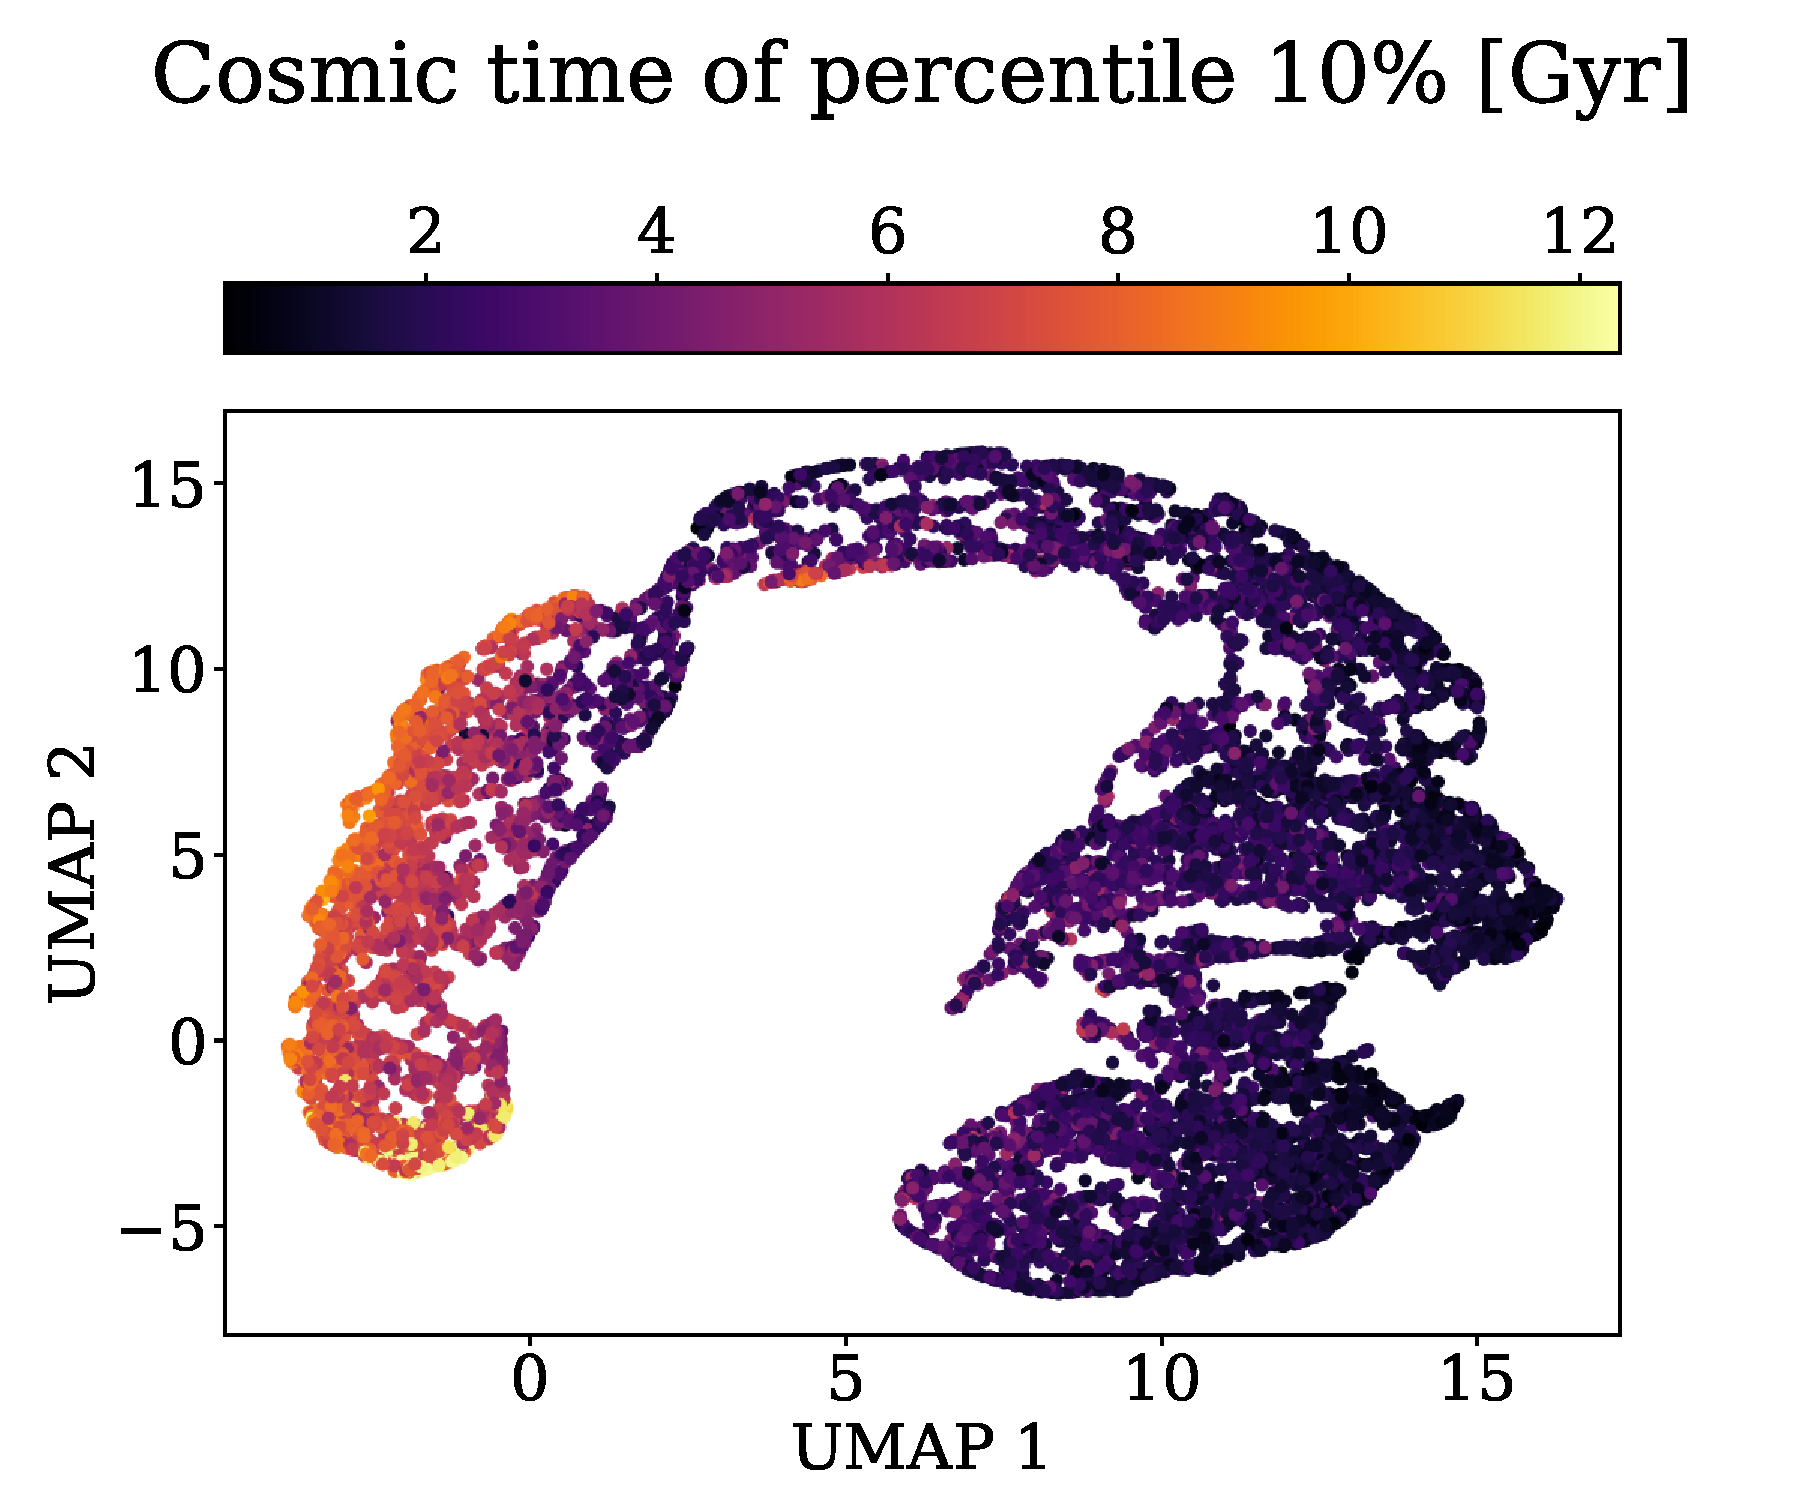
\includegraphics[width=0.33\textwidth]{images/latents/UMAP_10.pdf}
    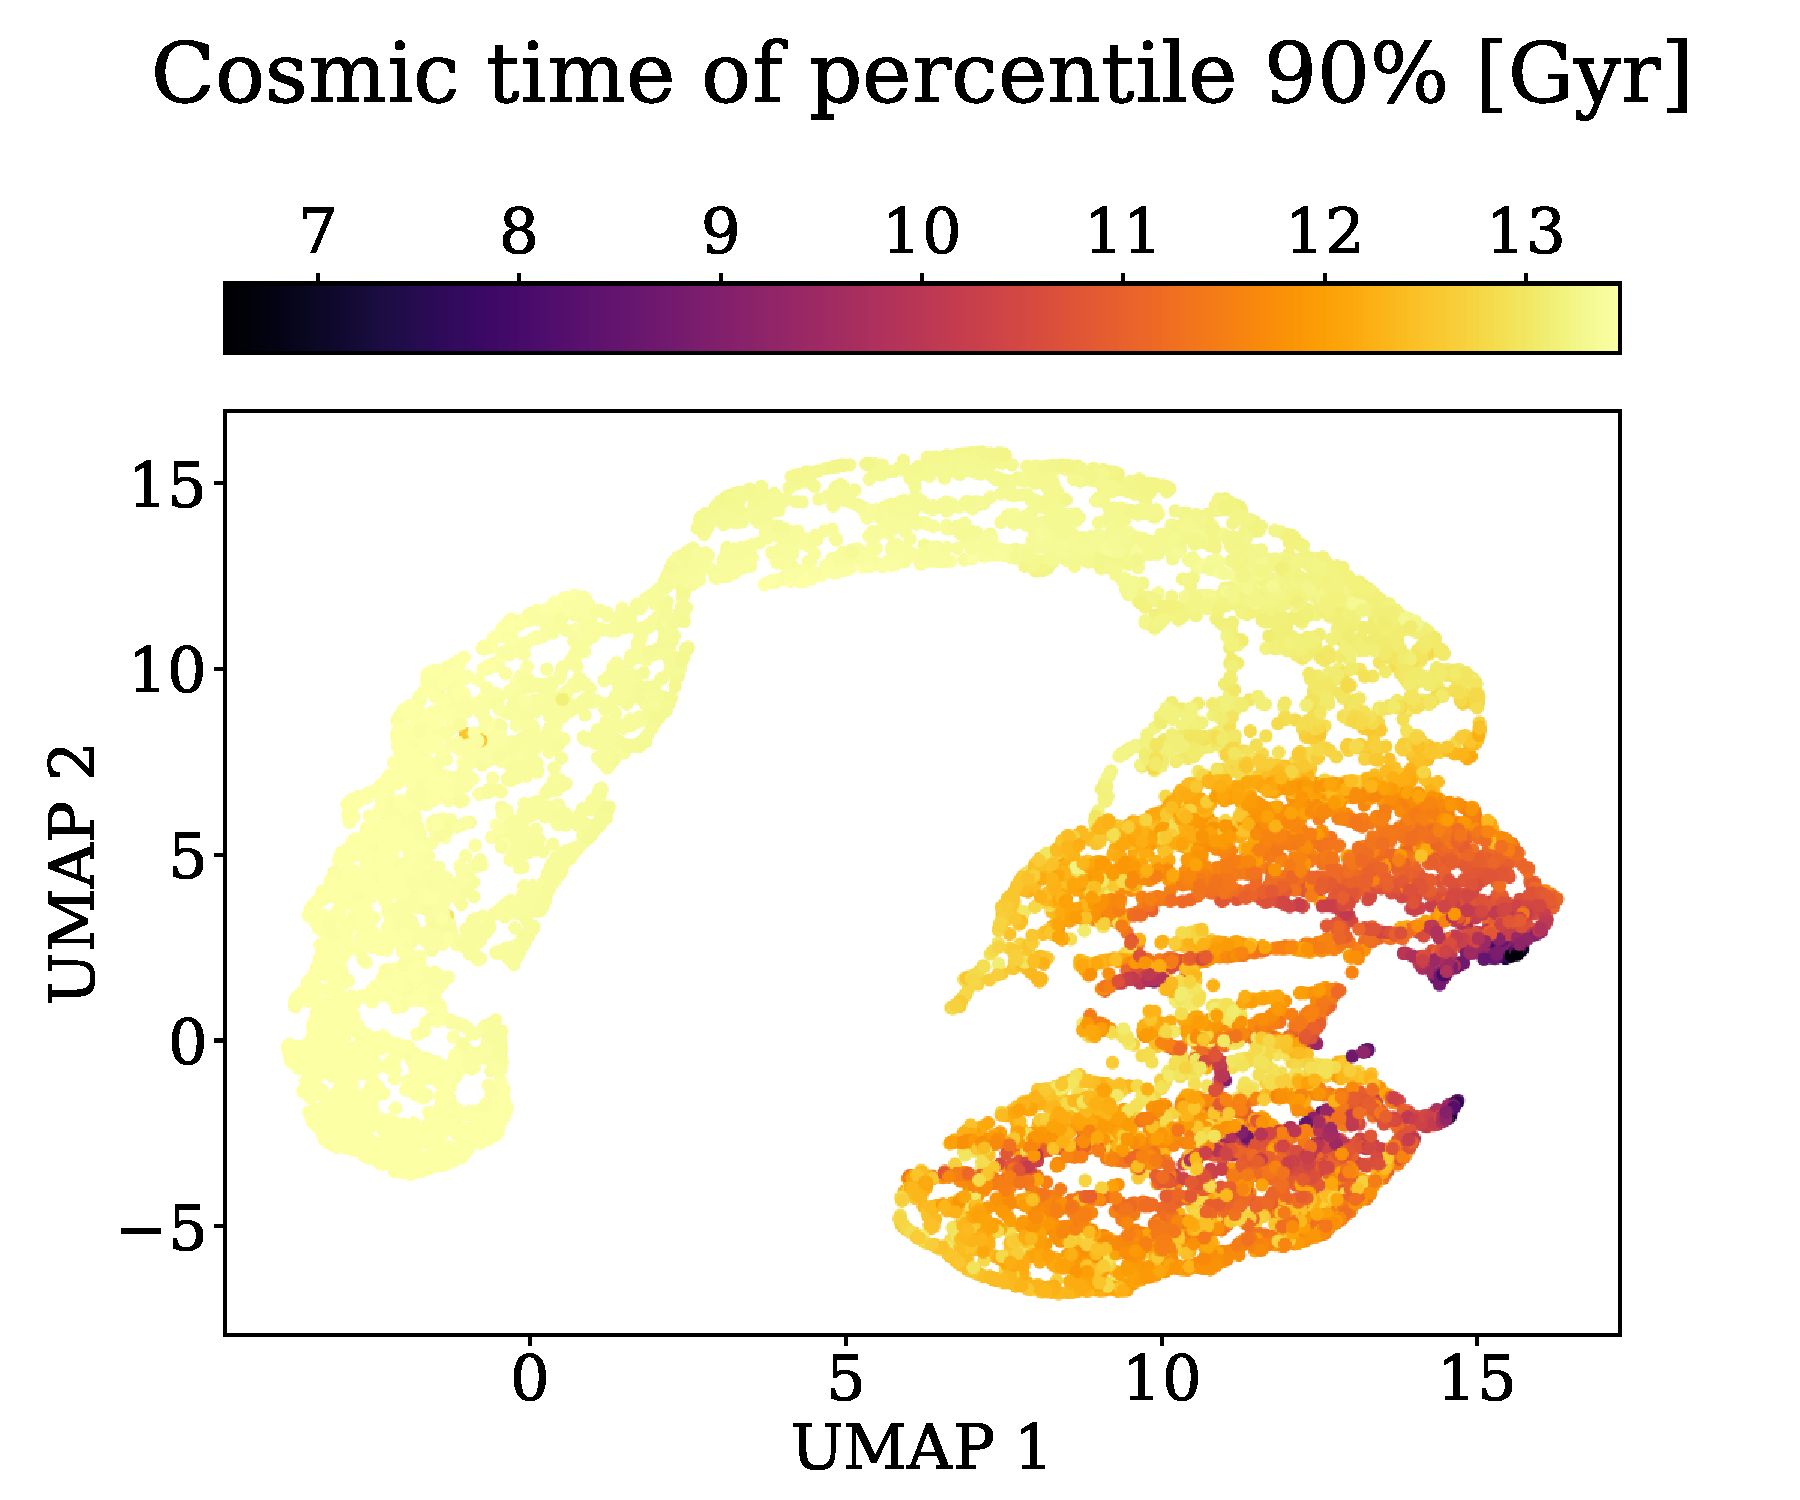
\includegraphics[width=0.33\textwidth]{images/latents/UMAP_90.pdf}
    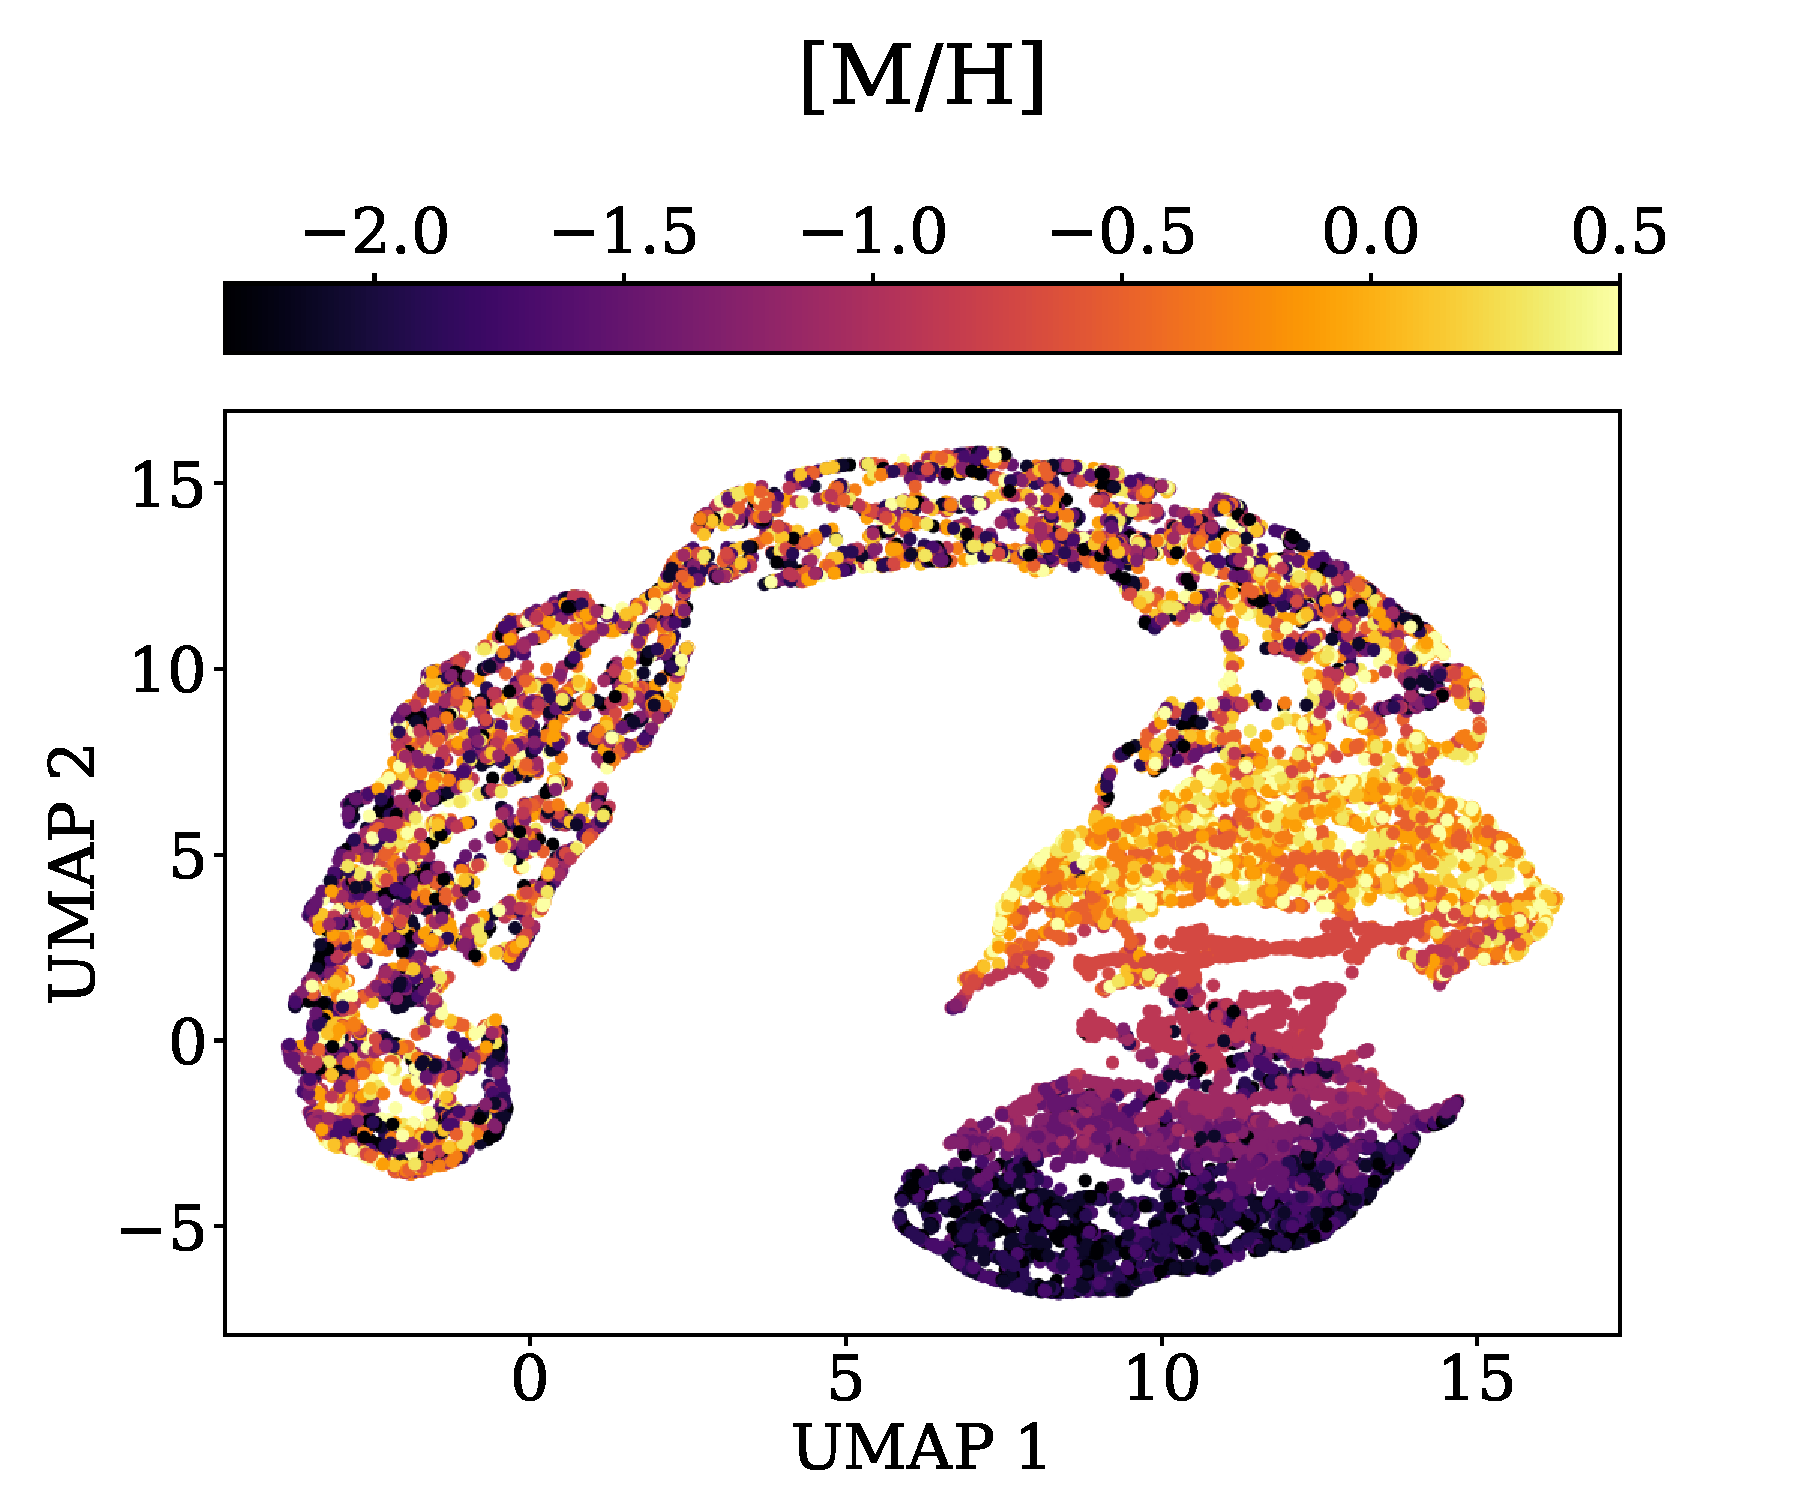
\includegraphics[width=0.33\textwidth]{images/latents/UMAP_met.pdf}
    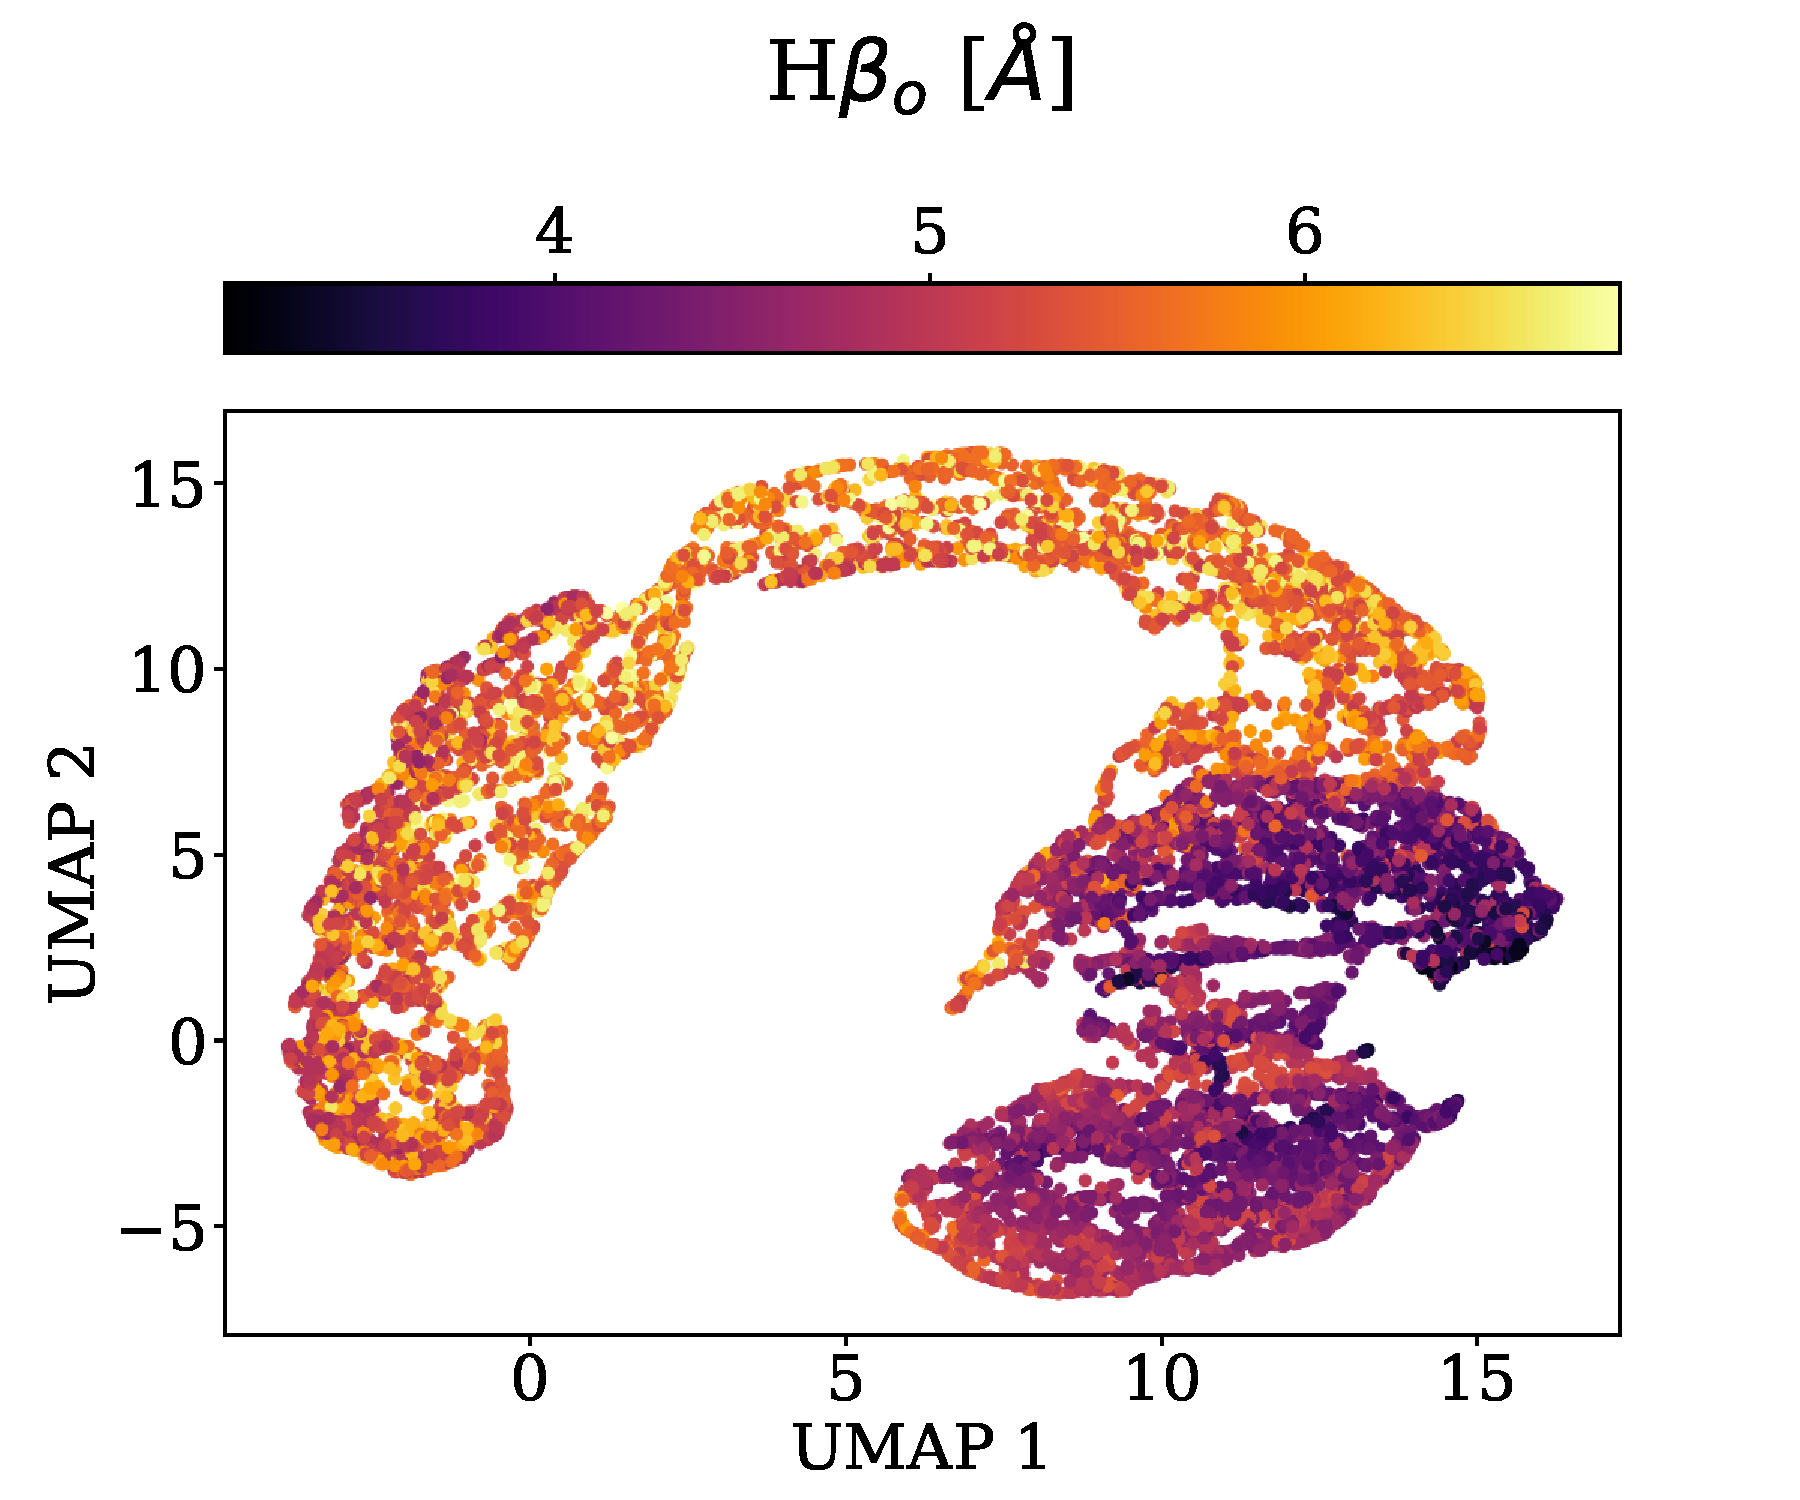
\includegraphics[width=0.33\textwidth]{images/latents/UMAP_hbeta.pdf}
     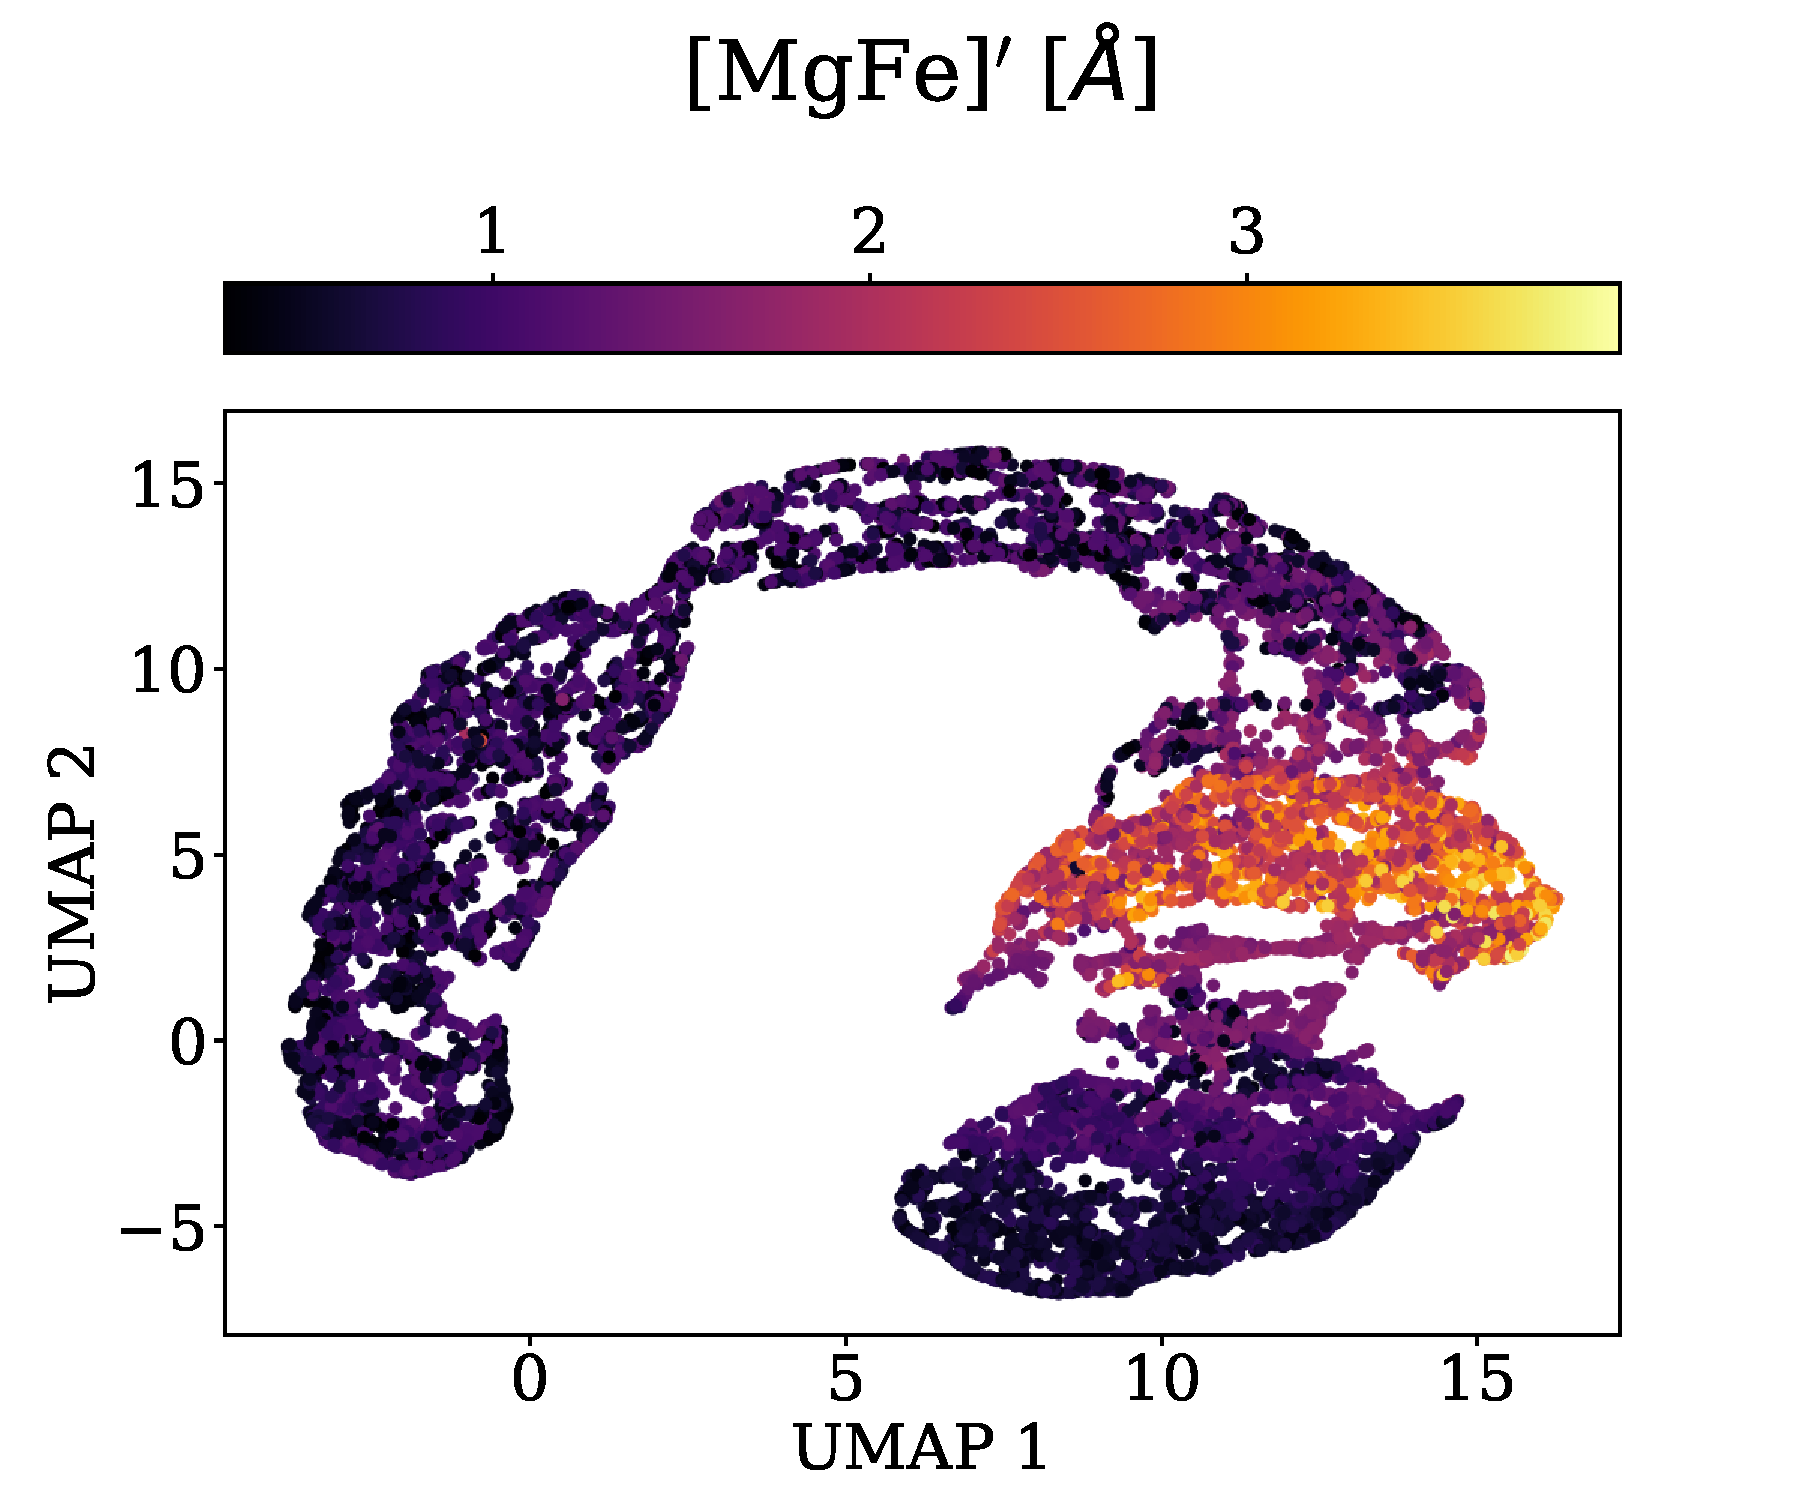
\includegraphics[width=0.33\textwidth]{images/latents/UMAP_mgfe.pdf}


     
    \caption{UMAP embedding for the latent representations. Each dot corresponds to a synthetic galaxy from the test sample. The closer two galaxies are on the map, the more similar are their latent representations. Different colourmaps are set according to the cosmic time at which the percentiles $10\%$ (top left) and $90\%$ (top middle) of the total stellar mass are reached, $[\rm{M/H}]$ (top right), and the two line indices  $\rm H{\beta_{o}}$ (lower left) and $[\rm{MgFe}]^{\prime}$ (lower right). Clear trends can be observed, demonstrating that the information encoded in the latent vectors is optimal for recovering the SFHs and metallicities.}
    \label{umap}
\end{figure*}



\subsection{Recovering SFHs of synthetic galaxies}
\label{post}
The network is trained with $90$\% of the generated samples ($x=$ {latent vectors}, $y=$ {nine stellar mass percentiles, $\rm{[M/H]}$}), with $10\%$ of these composing the validation set. Once the training is finished ($\sim4$ hours: $1$ hour for the encoder and $3$ hours for the Normalising Flows), the remaining $10$\% of the samples is used to test its performance, by obtaining probability distributions for the values of each percentile and $\rm{[M/H]}$ from their latent representations, and comparing the distributions with the true values. Each posterior estimation for the test set is performed with $1{,}000$ samples, taking $\sim0.4$\,s to get the predictions for the $10$ quantities of each galaxy. All the time estimations have been made using a NVIDIA Tesla P100 PCIe GPU with 12GB.\\



Figure \ref{examples} shows five examples of synthetic SFHs from the test set. The true values for the mass percentiles are indicated with  solid lines, while the recovered median of the posterior is shown with dashed lines. Light- and dark-shaded areas indicate the one and two $\sigma$ confidence intervals. It its clear that the model can recover from the latent vectors SFHs that are fully consistent with the ground truth within the expected uncertainties. In Fig.~\ref{meanvstrue}, we plot the median values of the posterior distributions predicted for the $15{,}000$ test galaxies against the true values, for the percentiles $10\%$, $50\%$, $90\%$ (in cosmic time), and for the metallicity. Both agree, close to the one-to-one relation, reaching high $R^{2}$ values\footnote{Also known as coefficient of determination $\displaystyle R^2=1-\frac{\sum_{i=1}^n\left(y_i-\widehat{y}_i\right)^2}{\sum_{i=1}^n\left(y_i-\overline{y_i}\right)^2}$, not to be confused with the square of the Pearson's coefficient.} of $0.88$, $0.97$, $0.98$, and $0.96$, respectively.  A larger scatter is observed for earlier percentiles, which is expected as the luminosity of young stars `outshines' the spectra, hiding the information of the oldest ones. \\

Posterior distributions for the percentiles $10\%$, $50\%$, $90\%$, and for the metallicity are shown as a corner plot in Fig.~\ref{corner}, for a single galaxy from the test set. The posteriors have been sampled with $1{,}000$ realisations. They deviate slightly from Gaussian functions, showing multimodalities associated with the degeneracy between the age (in particular the percentile $90\%$)  and  the metallicity, but in perfect agreement with the true values, indicated with solid lines.\\


Figures \ref{examples}, \ref{meanvstrue} and \ref{corner} confirm that the model is indeed capable of recovering the stellar mass growth and metallicity with uncertainties associated with the complexity of the inversion problem, due to the very nature of the spectra and to the observational imprints left by galaxies on them.  \\



\begin{figure}[t]
    \centering
    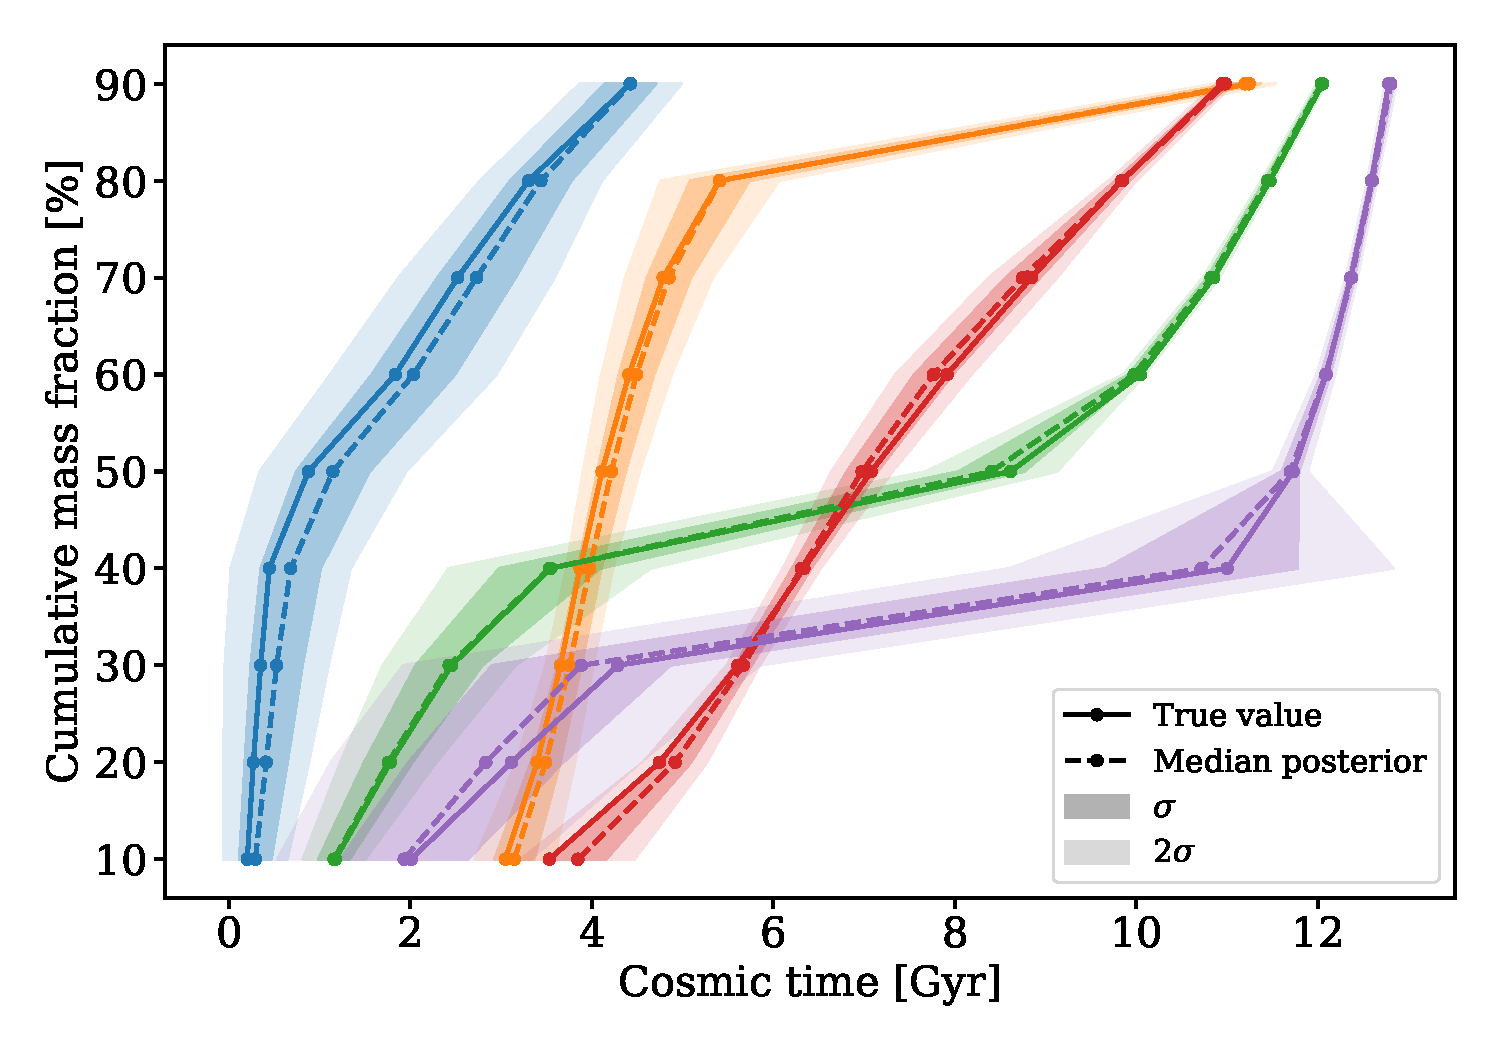
\includegraphics[width=0.49\textwidth]{images/posterior/cummul_mass_growth_2.pdf}
    \caption{Percentile predictions for five synthetic galaxies. The cumulative mass curves indicate the time at which the nine stellar mass percentiles are achieved over cosmic time. The solid lines correspond to the true values and the dashed ones to the predictions (medians of the posterior distributions). The $\sigma$ and $2 \sigma$ intervals of confidence are shaded dark and light, respectively. The model performs reliable reconstructions for all five galaxies.}
    \label{examples}
\end{figure}

\begin{figure}[h!]
    \centering
    
    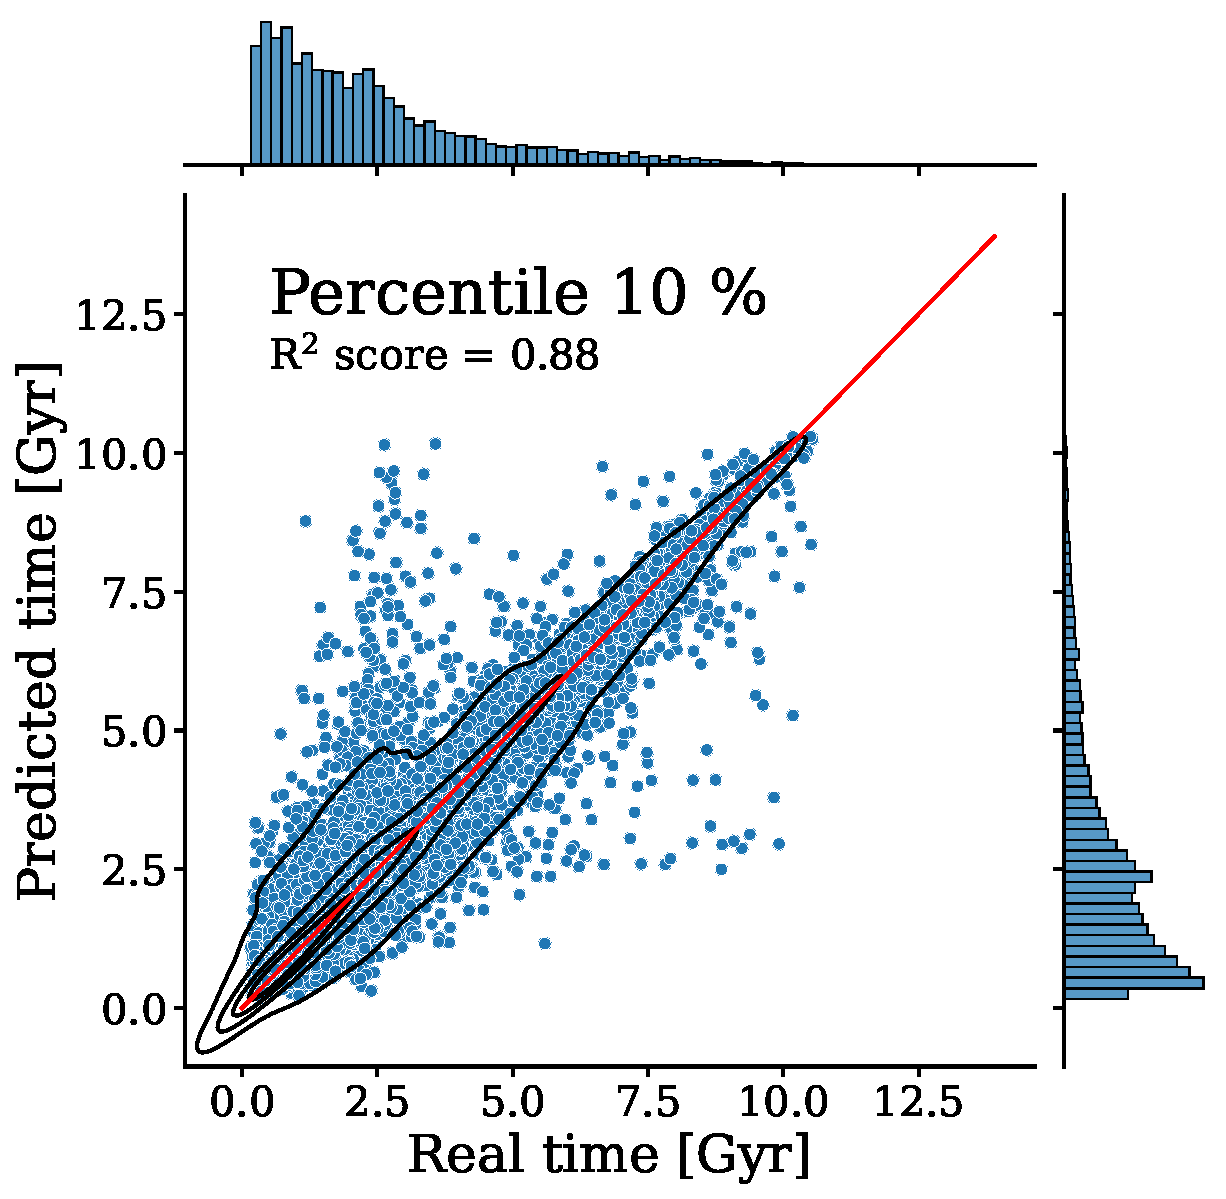
\includegraphics[width=0.285\textwidth]{images/posterior/sns_mean_true_0.pdf}
    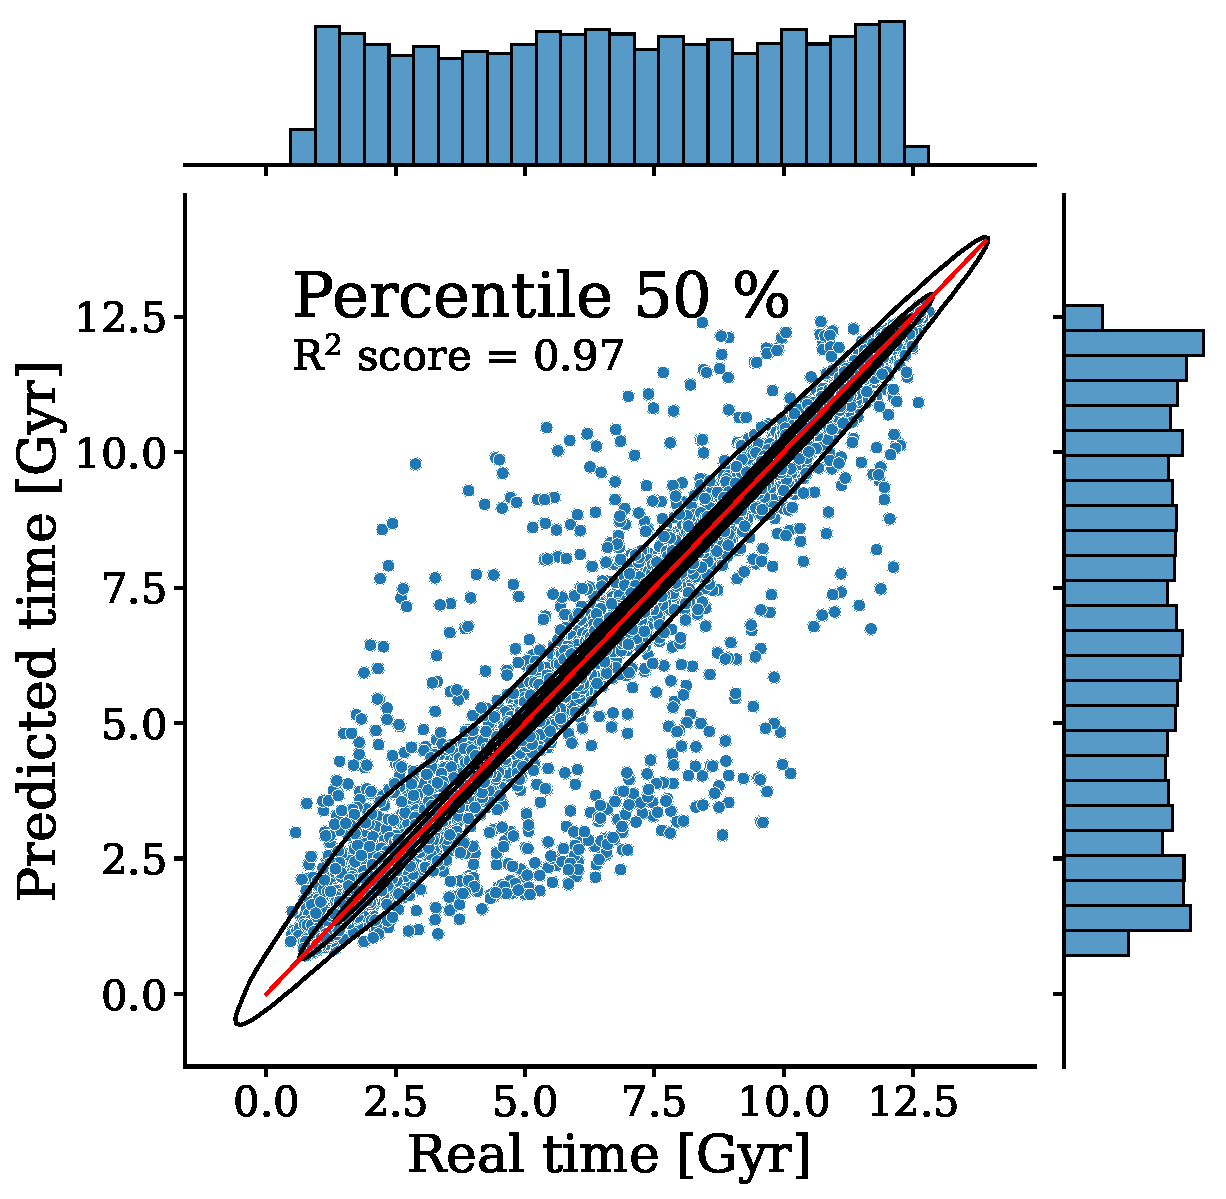
\includegraphics[width=0.285\textwidth]{images/posterior/sns_mean_true_4.pdf}
    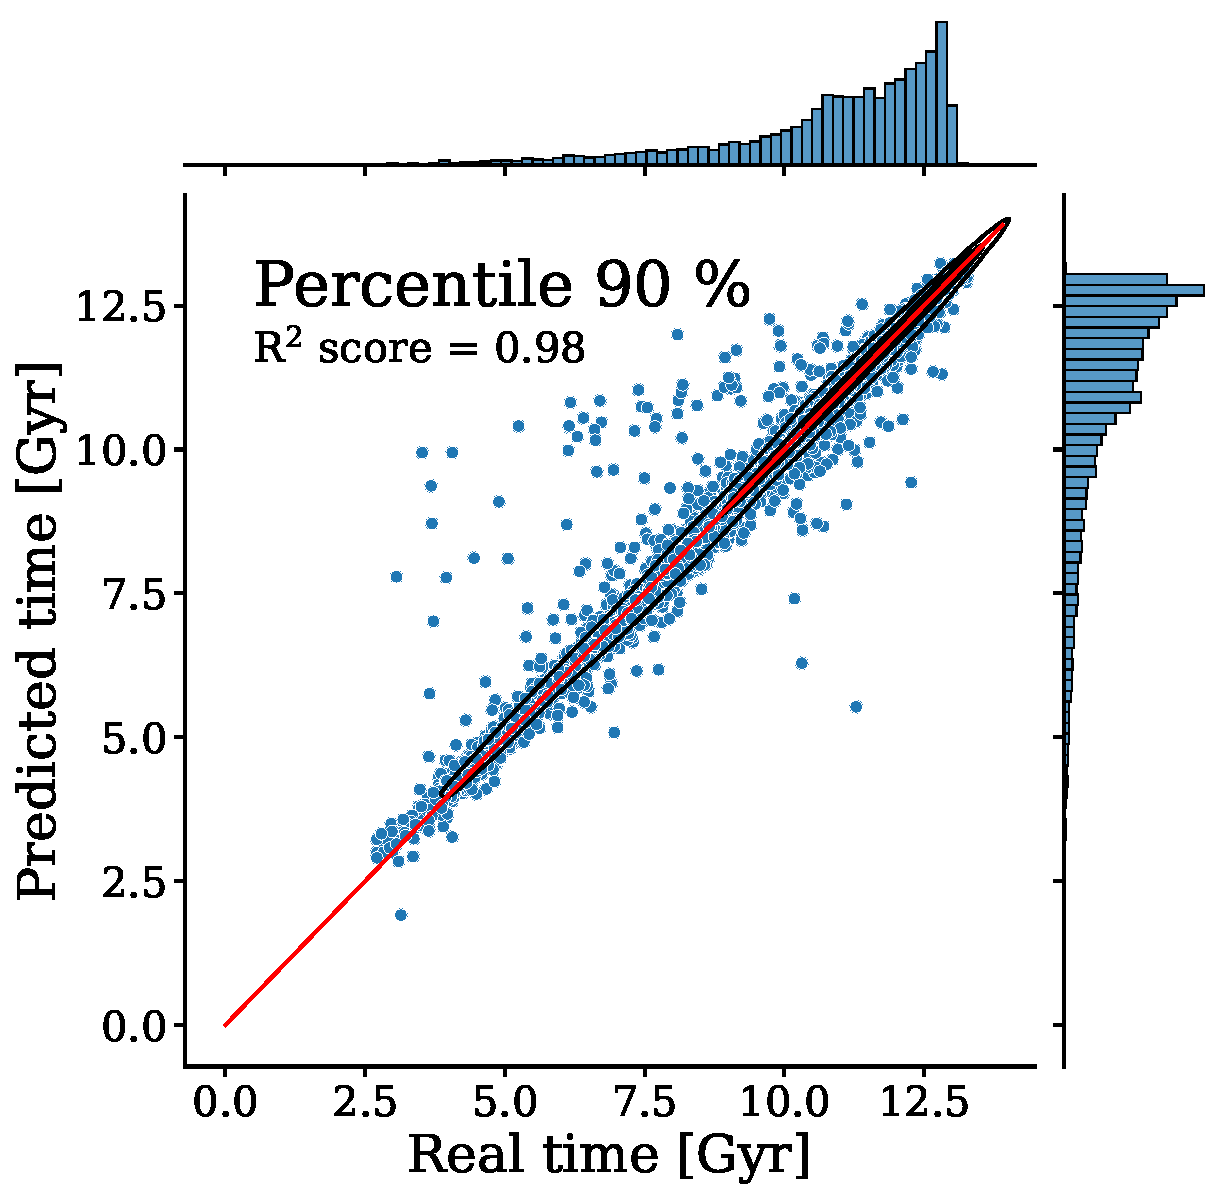
\includegraphics[width=0.285\textwidth]{images/posterior/sns_mean_true_8.pdf}
    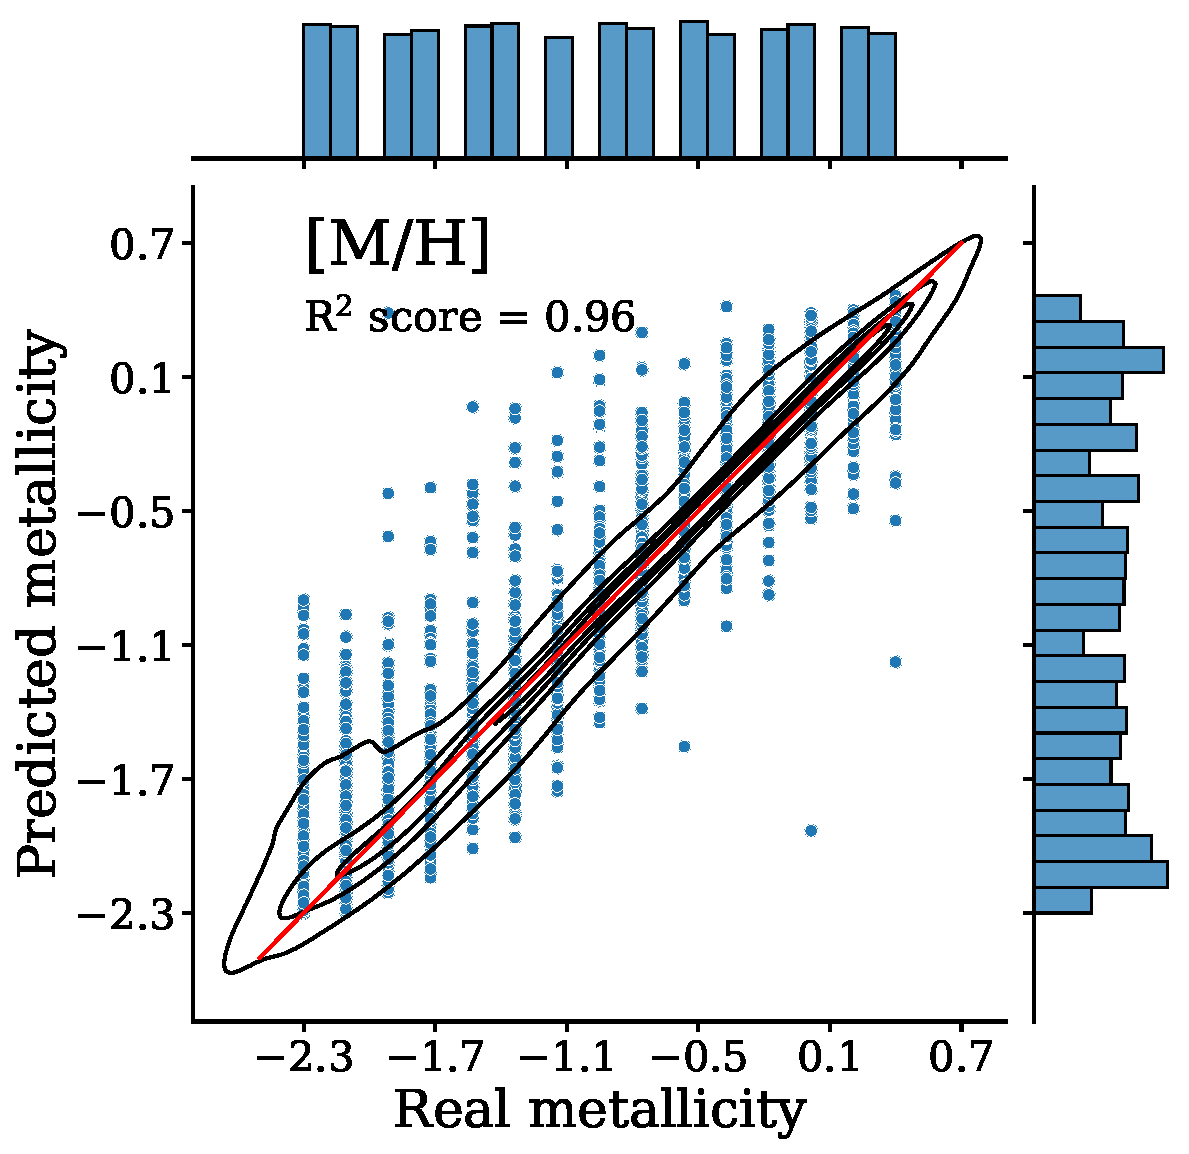
\includegraphics[width=0.285\textwidth]{images/posterior/sns_mean_true_9.pdf}
    
    \caption{Median values of the posterior distributions estimated for the percentiles $10\%$, $50\%$, $90\%$, and $\rm{[M/H]}$, compared to the true values. The $R^2$ score achieved for each prediction is $0.88$, $0.97$, $0.98$, and $0.96$, respectively. Each blue dot is a different sample from the test set. The red line shows the one-to-one relation, the histograms at the right of each panel show the marginal distributions of the predictions, and the histograms of the real data are shown at the top. Kernel Density Estimation (KDE)  contours are drawn in black at iso-proportions of the density of samples.}
    \label{meanvstrue}
\end{figure}



\begin{figure}[h!]
    \centering
    
    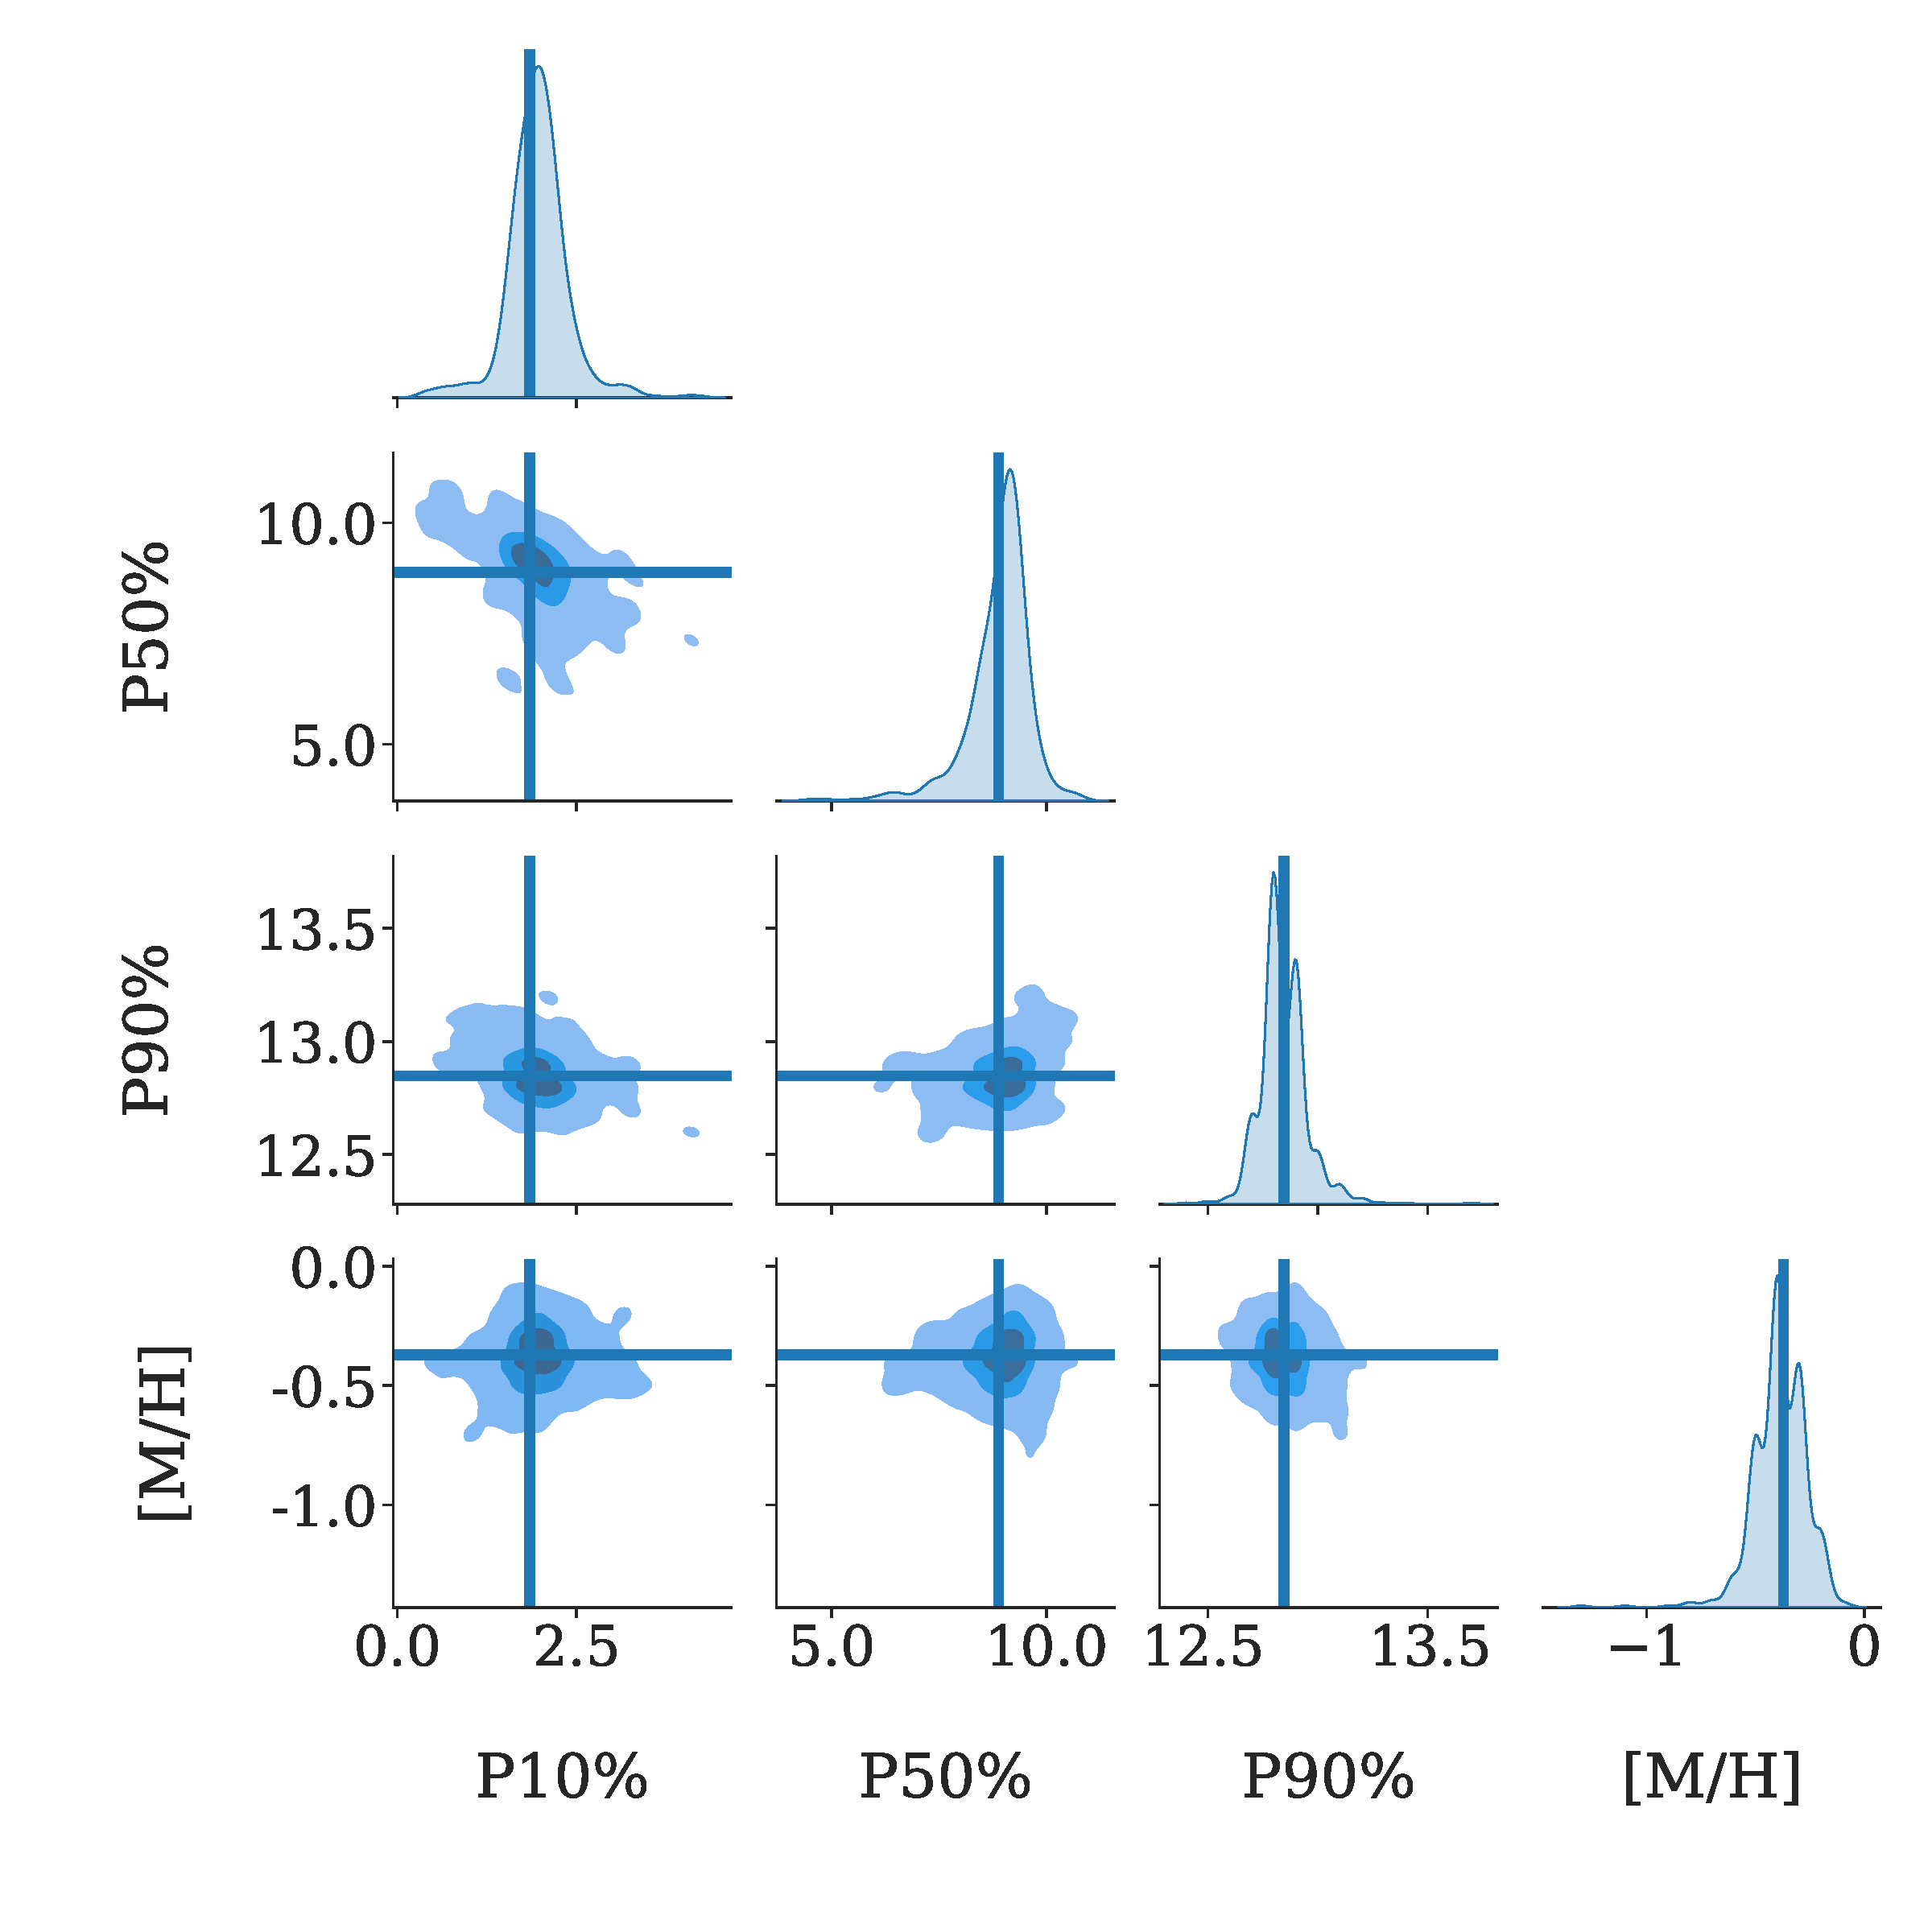
\includegraphics[width=0.5\textwidth]{images/posterior/conerplot0_ok.pdf}

    \caption{Corner plot with the posterior distributions for a simulated galaxy, sampled with $1{,}000$ realisations for the percentiles $10\%$, $50\%$, $90\%$, in Gyr, and for $\rm{[M/H]}$. KDE contours are drawn with different shades at iso-proportions of the density of samples. The solid lines correspond to the true values.  The distributions deviate slightly from Gaussian functions, showing  multimodalities associated with the degeneracy of the parameter space, but in perfect agreement with the true values. }
    \label{corner}
\end{figure}

\subsection{Simulation-based calibration}
\label{sbc}
A key point is ensuring that the estimated posterior distributions are well calibrated. We use simulation-based calibration (SBC) as described in  \cite{talts2020validating} to examine the distribution of the rank statistics of the true parameter values withing the marginalised posteriors, which must be uniform if the posterior samples are consistent with the prior. The only requirement of this test is that we have a generative model for our data, so that we are able to obtain observations from the predicted posteriors of the physical parameters. This is not exactly true in our case, since we obtain a SFH sampled with nine time bins (the percentiles) instead of $1{,}000$, as used during the forward model. For this reason, and with the only purpose of carrying out this test, we repeat the model training  with a simulation that only takes into consideration the percentiles, performing the linear combination with nine spectra, so that with the posteriors provided by the model we are able to recover directly the synthetic observations.\\

Figure \ref{ranks} shows a histogram from an ensemble of rank statistics of $1{,}000$ prior samples relative to the corresponding posterior samples,  for the percentiles $10\%$, $50\%$, $90\%$, and for $\rm{[M/H]}$. Each histogram is complemented with a grey band indicating $99\%$ of the variation expected from a uniform histogram. Additionally, in Fig.~\ref{ecdf} we include the empirical cumulative distribution function (CDF), together with the diagonal expected from a well-calibrated posterior. Both plots show uniformly distributed ranks, and consequently an optimal overall performance, except for the metallicity, where we detect a slight $\cap$ shape. This symmetric deviation, related with the wide binning of $\Delta\rm{[M/H]}=0.1929$ we use throughout the work\footnote{A finer binning is always possible, but at the cost of a larger training set and longer training time.}, implies that the computed posterior will be wider than the true posterior, allowing us to estimate an upper limit for the uncertainty of the parameter.






\subsection{Testing with observations}

\label{obs}

To test the method we compare our measurements for $18$  stacks of early-type galaxies at $z \sim 0$ from SDSS spectra (with velocity dispersion in the range $100-320$ km/s), whose stellar populations have been studied in detail in \cite{La_Barbera_2013}. We highlight that the main advantage of working with these stacks is their very high S/N, and the absence of emission features, important because no noise models or emission lines have been incorporated in the simulation.\\

First, we convolve all the observations to emulate the maximum velocity dispersion of the dataset. Then, we clip the wavelength range to $[4023,6000]$ $\AA$, the maximum window that is common to all stacks. We also process the MILES spectra used for training to simulate the conditions of the observations. Once all the artificial spectra have the same resolution and wavelength range as the observations, we repeat the training, and then test the model performance again, analysing the impact of these changes on the performance.\\

As a result of the processing, the $R^2$ score on the synthetic test set decreases to $0.72$, $0.95$ and $0.96$ for the estimation of the percentiles $10\%$, $50\%$ and $90\%$, respectively, and to $0.96$ for the metallicity. These losses in performance, mainly for the first percentiles, are a direct consequence of reducing the resolution in the spectral lines, and clipping the Balmer jump in the bluer region of the spectra.\\




We then apply the trained model to the spectra of the stacks, sampling the posteriors with $10{,}000$ evaluations. In Fig.~\ref{percentiles_obs_full}, we show the median values of the measured distributions for the mass percentiles, as a function of cosmic time and redshift\footnote{Assuming a Planck13 cosmology \citep{planck13}.}, using a colourmap based on the velocity dispersions. The most massive galaxies (highest velocity dispersions) build up their stellar masses more abruptly, up to 90\% of their total stellar mass $1$ Gyr after the Big Bang, while the growth of stellar mass is softened as we move to less massive ones.\\ 

For a more detailed analysis, the median values of the posterior predictions, together with their uncertainties given by one standard deviation, are included in Table~\ref{table_obs}, for all $18$ observations. The quantities shown are the times by which $10$\%, $50$\% and $90$\% of the total stellar mass have been formed, as well as the metallicity. We do not find a clear trend between the metallicity and the velocity dispersion, but the margin of uncertainty is too large to make any further assumptions, mainly due to the wide binning in $\rm{[M/H]}$ of $0.1929$\,dex for the simulated sample. This is consistent with the results of \cite{La_Barbera_2013}, who reported a variation of $\sim 0.2$\,dex in metallicity from the least massive to the most massive stack.\\




Finally, we carry out a spectral reconstruction with our model in Fig~\ref{spectra_obs}, for the stacks with velocity dispersion $105$, $205$ and $300$ km/s. This test is usually referred to as Posterior Predictive Check (PPC,  \citealp{talts2020validating}), and allows us to verify that our measurements are indeed compatible with the observed spectra. These observed and reconstructed spectra must be close to each other in the latent space, but a priori this proximity is not trivial in the wavelength space, since we do not minimise the differences with respect to the observed spectra as in more traditional approaches, but perform the Bayesian inference on the latent representations. Even so, it is the most direct way we have of determining the  reliability of the measurements, and we do it by performing a linear combination of nine SSP MILES spectra of ages obtained from the percentiles of stellar mass, and metallicity fixed and equal to the predicted value. According to the definition of the percentiles, all nine spectra are weighted with $1/9$. The results are very positive, showing mean residuals of  $1.7\%$ between the fit and the observations, averaging over all $18$  stacks and wavelengths. The uncertainties are propagated into the spectra, within the grey-shadowed stripe in Fig~\ref{spectra_obs} corresponding to the interval of two standard deviations.

\subsection{Comparison with existing codes}
%to complete
\label{compare_ppxf}

We include another reconstruction of the spectra in Fig~\ref{spectra_obs}, namely a linear combination of MILES templates of  $34$ different ages and $12$ different metallicities ($408$ templates in total), where the weights are given by pPXF \citep{ppxf}. For a fair comparison, we use the same wavelength range as before without any continuum correction. The average of the residuals between the observed spectra and the pPXF fitting is $1.5 \%$. The observed spectra, our reconstructions from the percentiles and the reconstructions made with the weights of pPXF are in close agreement, not only in the latent space, but also in the wavelength space. We find that our method generally fits the spectra as accurately as pPXF despite, again, not being designed to reproduce them.\\

 On the other hand, the pPXF fitting takes $\sim30$ s for each stack, and since it does not provide an uncertainty, this measurement would be equivalent to a realisation of the posteriors obtained with our model, which take $4 \cdot 10^{-4}$\,s per stack.  Thanks to this acceleration of five orders of magnitude, our model can easily produce $10^3$ or $10^4$ samples of the posteriors for each observation and thus, always under the assumptions of the simulation, obtain a proper calibration of the uncertainty.


%time and deal with uncertainties in pPXF




\begin{figure*}[h!]
    \centering
    
    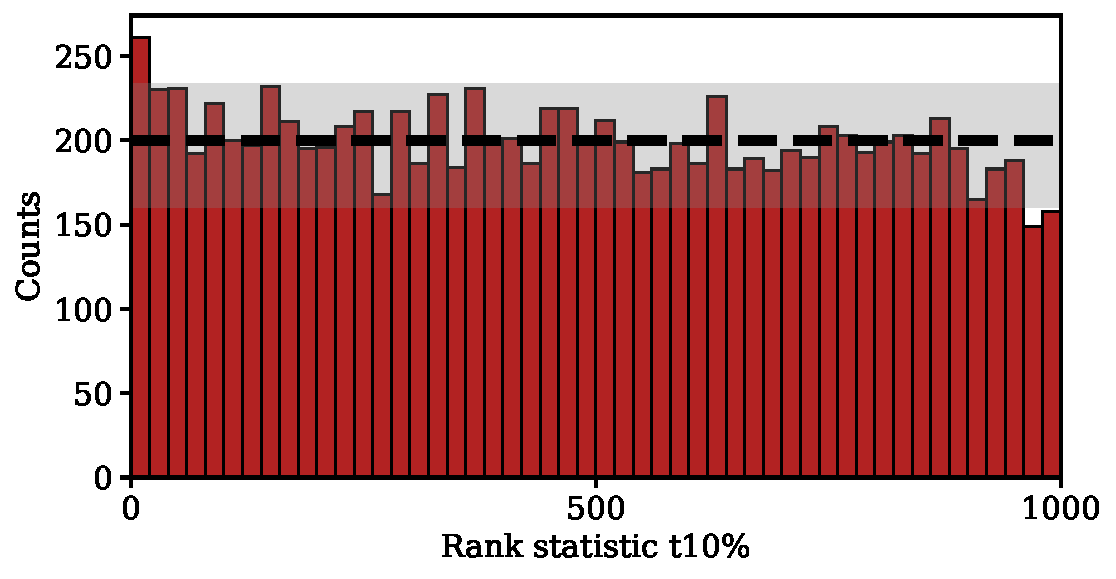
\includegraphics[width=0.45\textwidth]{images/sbc/rank_statisitic_1.pdf}
    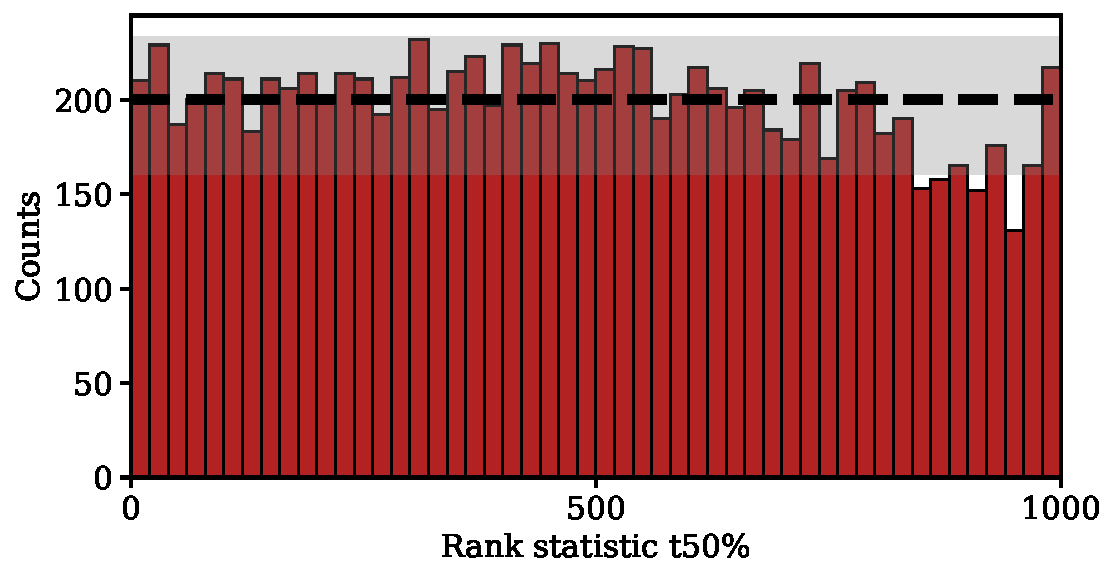
\includegraphics[width=0.45\textwidth]{images/sbc/rank_statisitic_2.pdf}
    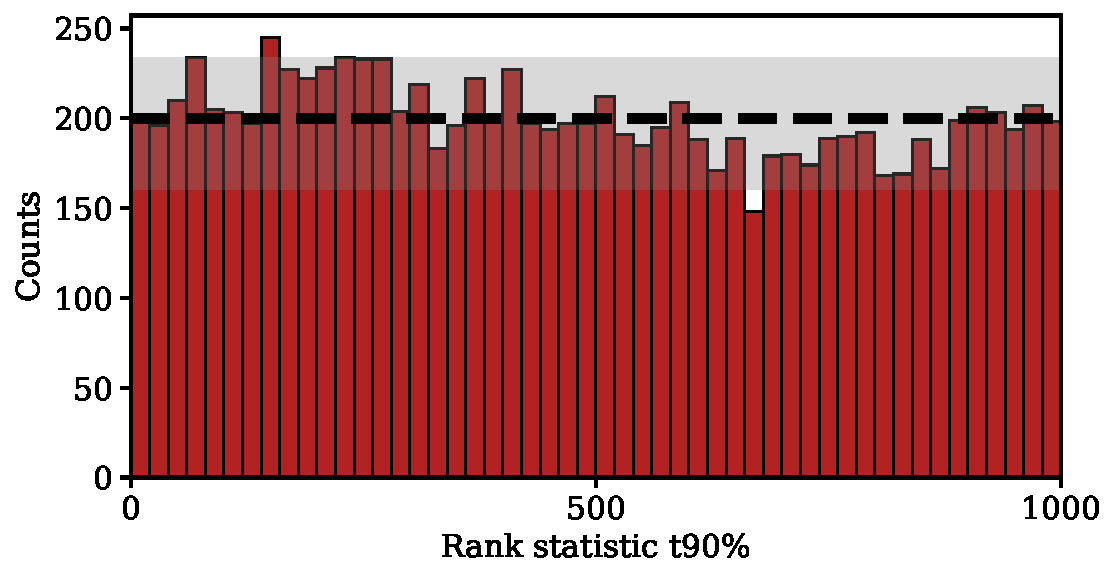
\includegraphics[width=0.45\textwidth]{images/sbc/rank_statisitic_3.pdf}
    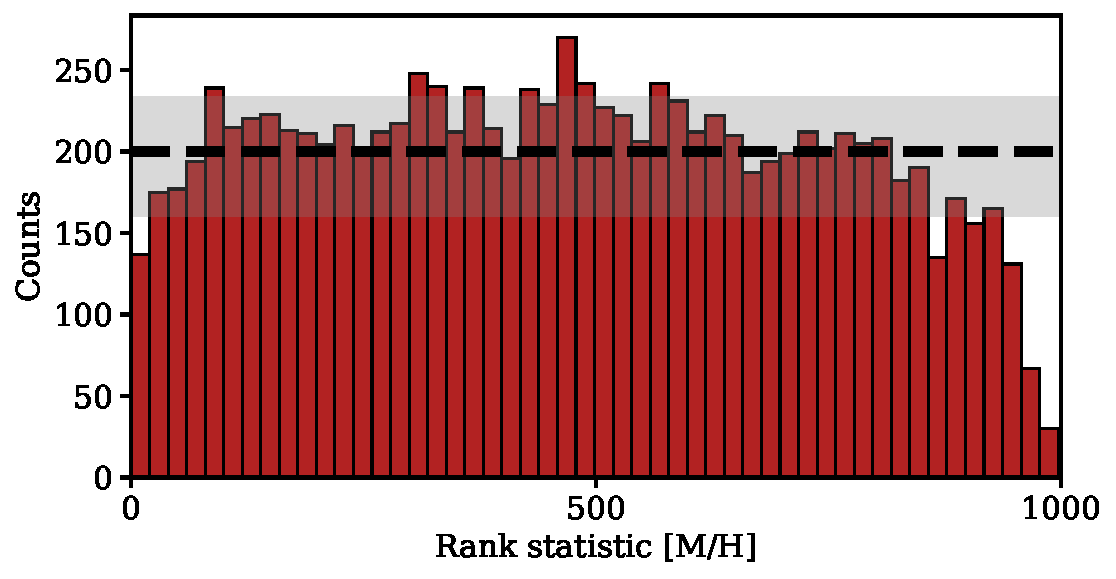
\includegraphics[width=0.45\textwidth]{images/sbc/rank_statisitic_4.pdf}
    
    
    
    \caption{Simulation-based calibration test of the posteriors for $1{,}000$ synthetic test observations. The red histograms in each panel represent the distribution of the rank statistic of the true value within the marginalised posterior for the percentiles $10\%$, $50\%$, $90\%$, and for $\rm{[M/H]}$. For a well calibrated posterior, the rank statistics will have a uniform distribution (black dashed line). A grey band indicates $99\%$ of the variation expected from a uniform histogram. The rank statistic distributions of our posteriors are nearly uniform for all of the four parameters, and therefore, the model provides unbiased and accurate posteriors.}

    \label{ranks}
\end{figure*}


\begin{figure}[h!]
    \centering
    
    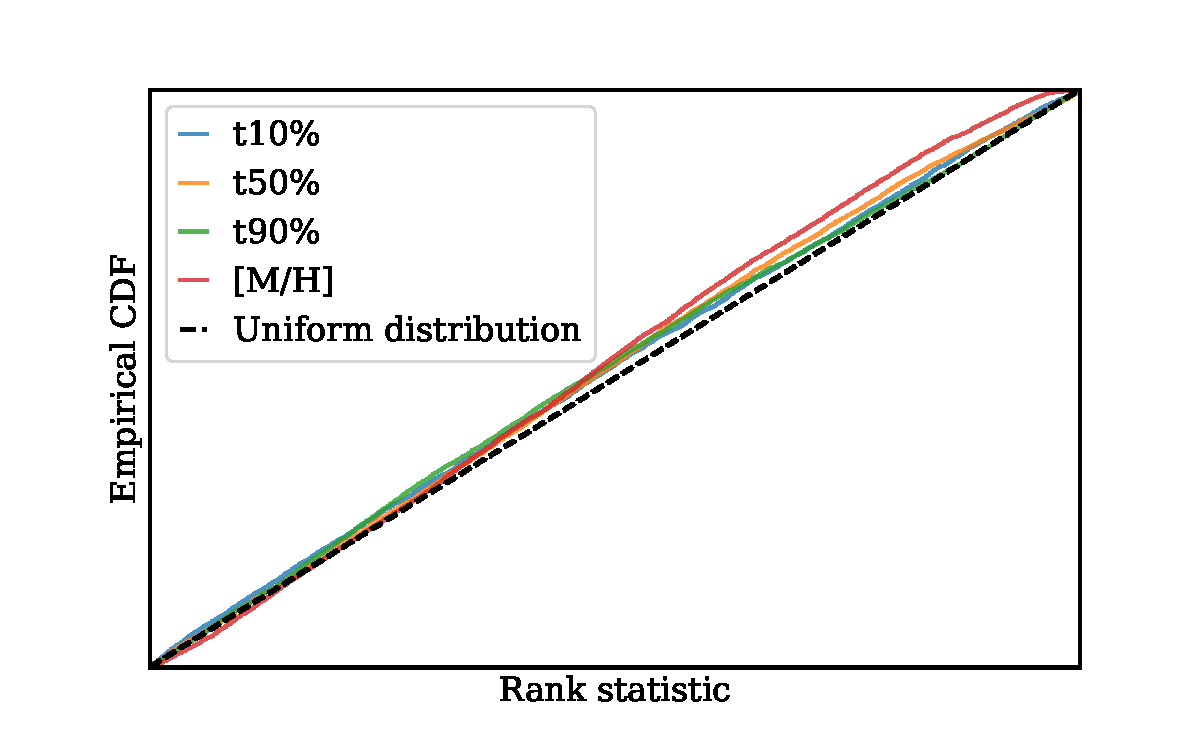
\includegraphics[width=0.5\textwidth]{images/sbc/ecdf.pdf}
    
    \caption{Empirical cumulative distribution functions (CDFs) for the percentiles $10\%$, $50\%$, $90\%$, and for $\rm{[M/H]}$, obtained with $1{,}000$ synthetic test observations.  If the posteriors are properly calibrated, the nominal coverage probability (percentage of probability volume), on the $x$-axis, would be equal to the coverage probability (percentage of actual values in such volume), on the $y$-axis, so the CDF is diagonal (black dashed line). Our CDFs are located very close to the diagonal, and the slight differences towards a conservative posterior, where the actual coverage probability is greater than the nominal coverage probability, allow the use of the model uncertainties as an upper limit. }

    \label{ecdf}
\end{figure}

\begin{figure}[h!]
    \centering
    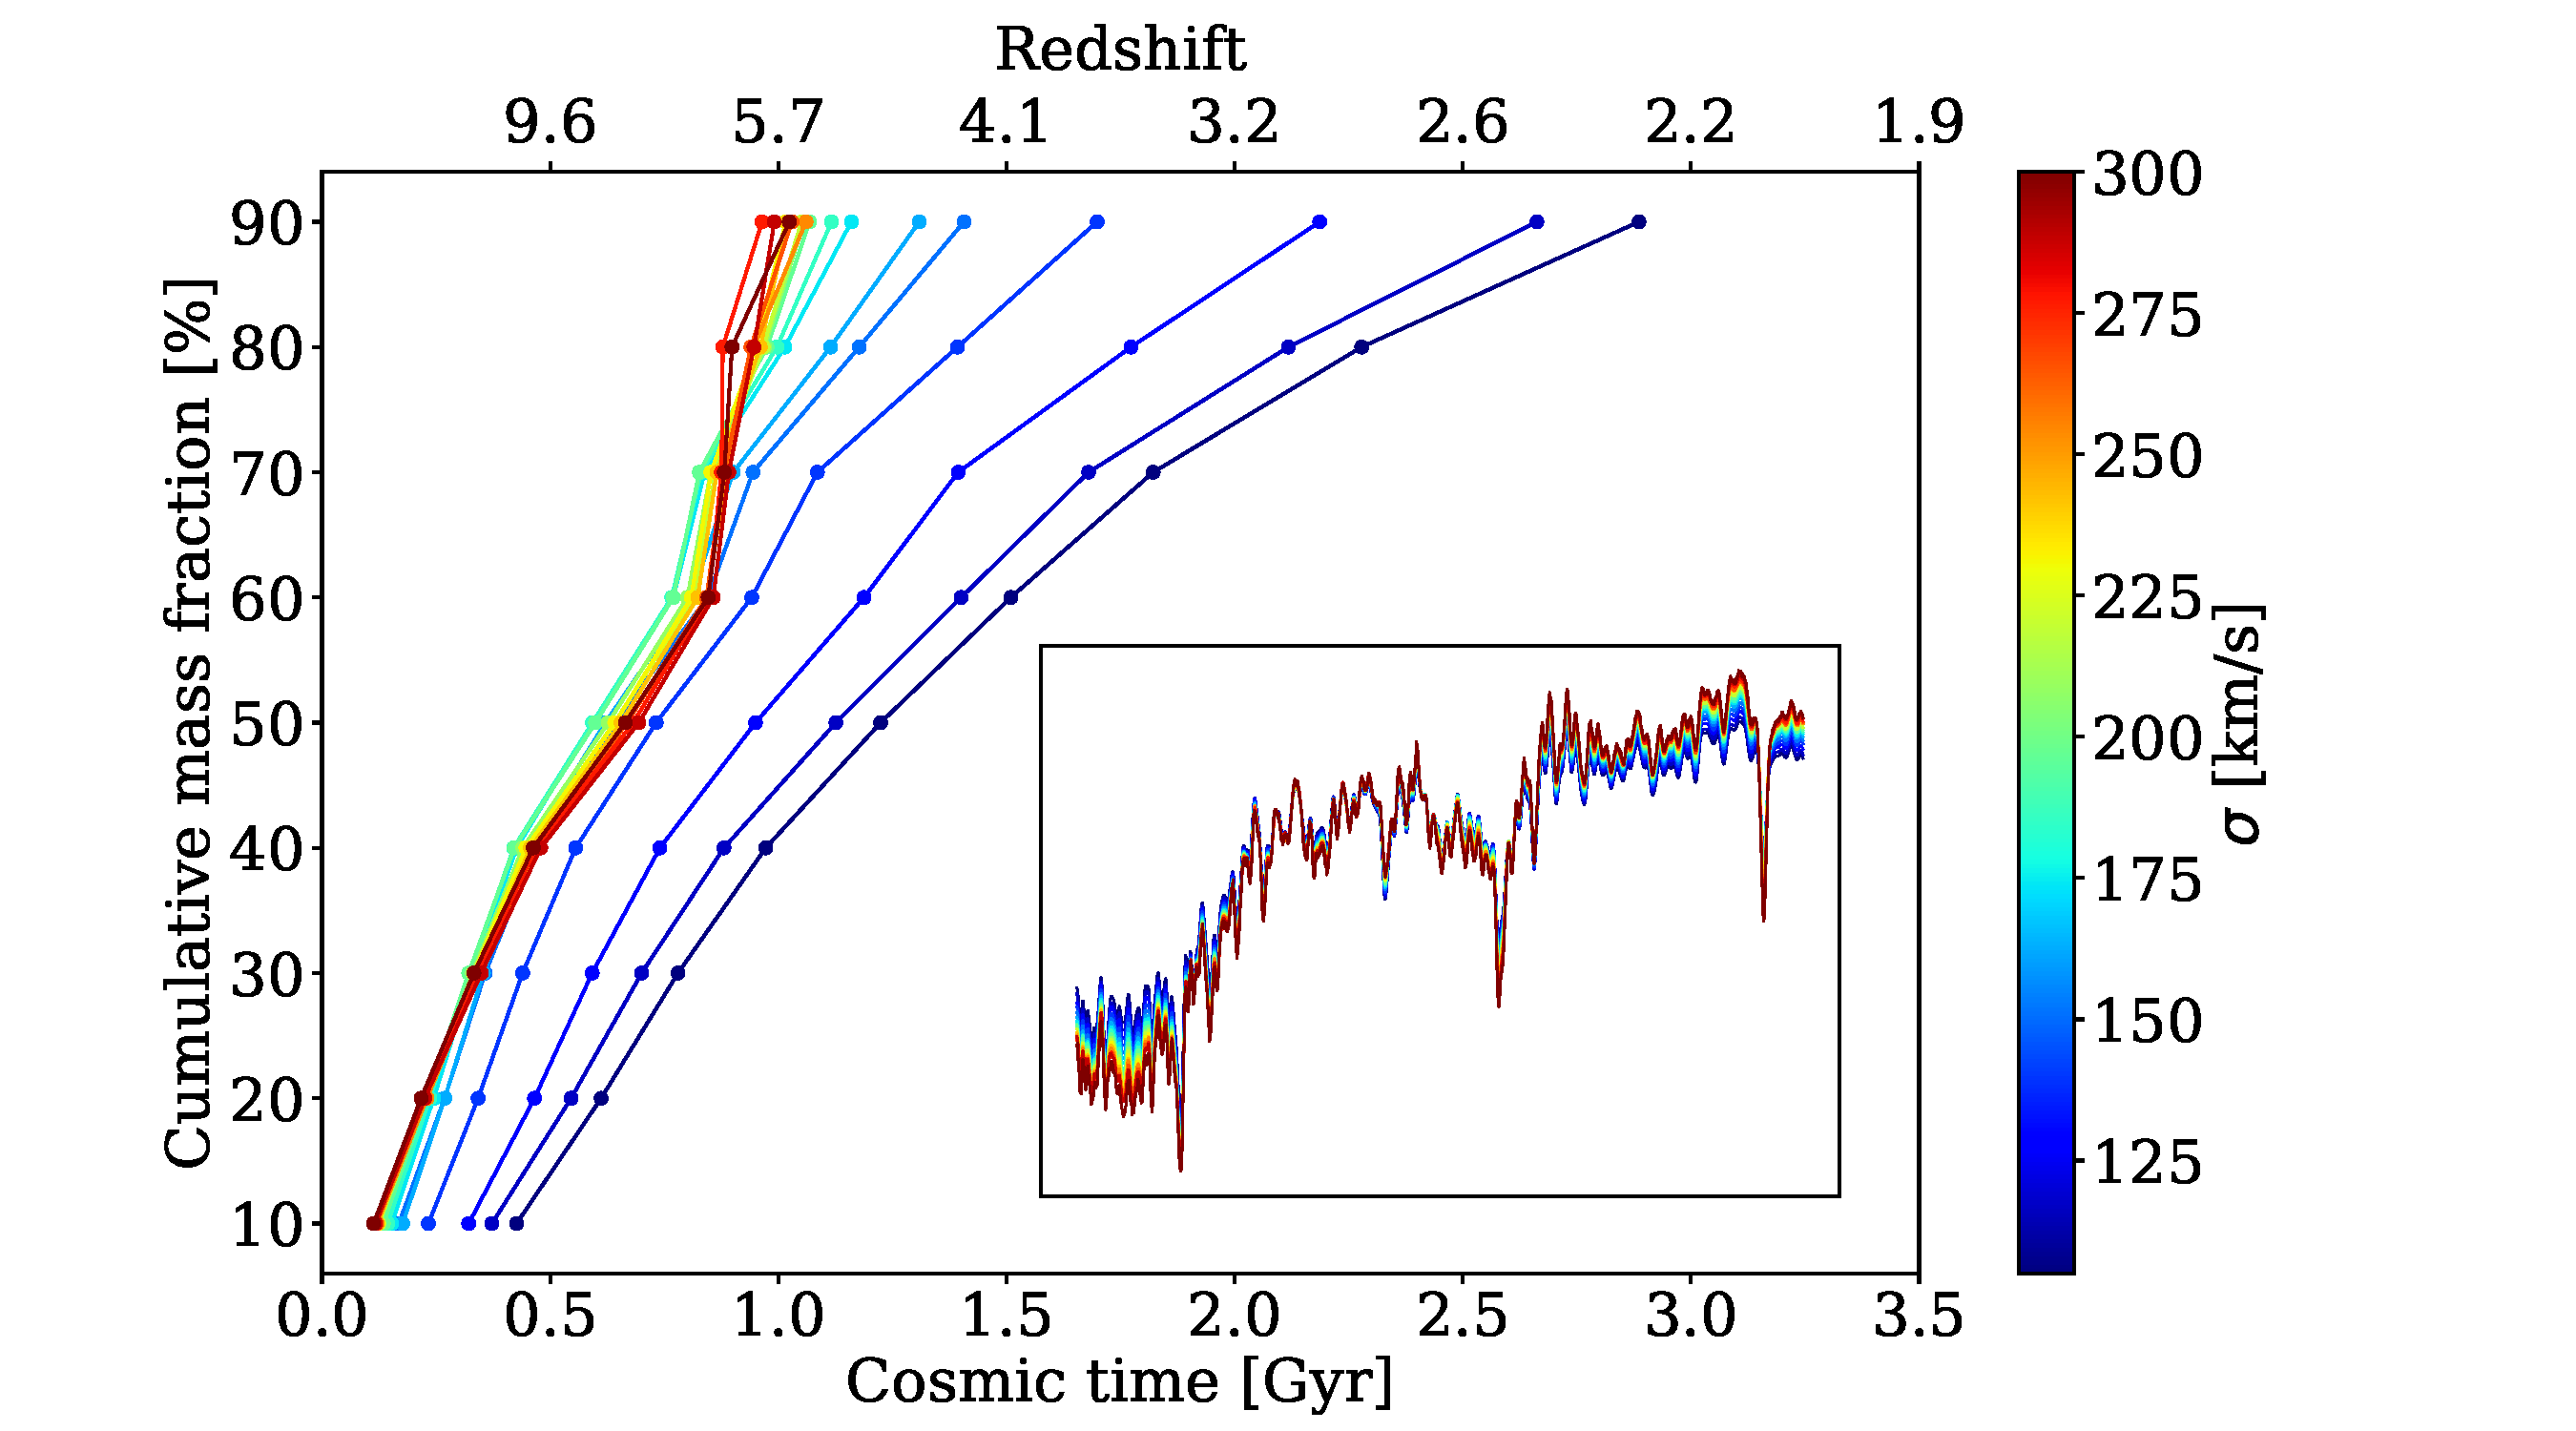
\includegraphics[width=0.5\textwidth]{images/obs/pred_gal_full.pdf}
    \caption{Median values of the posterior distributions obtained for the stellar mass percentiles of $18$ stacks, as a function of cosmic time in Gyr and redshift, coloured according to their velocity dispersions in km/s.  Redder colours are assigned to higher velocity dispersions (more massive galaxies), while bluer ones point to lower velocity dispersions (less massive ones). In the inset, we plot the observed spectra, normalised and in the wavelength range $[4023, 6000] \; \AA$, with the same colourmap.}
    \label{percentiles_obs_full}
\end{figure}



\begin{table}[h!]

\caption{Measurements of the model for 18 stacks with mean velocity dispersions in the range $105-300$ km/s. We include the cosmic time in Gyr at which $10$\%, $50$\%, and $90$\% of the total stellar mass are formed, as well as the metallicity $\rm{[M/H]}$. The values shown correspond to the median values of the predicted posterior distributions, and the uncertainties to the standard deviations.}
\centering
\resizebox{\hsize}{!}
            {
\begin{tblr}{
  cells = {c},
  hline{1,20} = {-}{0.08em},
  hline{2} = {-}{0.05em},
}

${\sigma}$ {[km/s]} & {P10\% [Gyr]} & {P50\% [Gyr]} & {P90\% [Gyr]} & $\rm{[M/H]}$ \\
100-110                            & 0.42$\pm0.22$         & 1.21$\pm0.34$        & 2.89$\pm0.63$        & 0.11$\pm0.24$   \\
110-120                            & 0.36$\pm0.22$        & 1.12$\pm0.32$        & 2.63$\pm0.66$        & 0.13$\pm0.23$  \\
120-130                            & 0.32$\pm0.21$        & 0.95$\pm0.33$        & 2.21$\pm0.75$        & -0.05$\pm0.32$ \\
130-140                            & 0.23$\pm0.17$        & 0.72$\pm0.29$        & 1.66$\pm0.70$         & -0.12$\pm0.40$  \\
140-150                            & 0.16$\pm0.13$        & 0.63$\pm0.24$        & 1.43$\pm0.57$        & 0.06$\pm0.38$  \\
150-160                            & 0.17$\pm0.13$        & 0.61$\pm0.25$        & 1.31$\pm0.61$        & -0.05$\pm0.39$ \\
160-170                            & 0.15$\pm0.12$        & 0.59$\pm0.21$        & 1.18$\pm0.54$        & 0.01$\pm0.40$   \\
170-180                            & 0.15$\pm0.11$        & 0.60$\pm0.21$         & 1.11$\pm0.53$        & -0.05$\pm0.40$  \\
180-190                            & 0.13$\pm0.10$         & 0.59$\pm0.20$         & 1.08$\pm0.50$         & -0.07$\pm0.41$ \\
190-200                            & 0.13$\pm0.09$        & 0.62$\pm0.18$        & 1.04$\pm0.46$        & 0.01$\pm0.37$  \\
200-210                            & 0.13$\pm0.11$         & 0.63$\pm0.16$       & 1.02$\pm0.41$        & -0.03$\pm0.39$  \\
210-220                            & 0.13$\pm0.10$         & 0.64$\pm0.17$        & 1.02$\pm0.44$        & -0.04$\pm0.37$ \\
220-230                            & 0.12$\pm0.09$        & 0.65$\pm0.15$        & 1.02$\pm0.42$        & -0.07$\pm0.37$ \\
230-240                            & 0.12$\pm0.12$        & 0.67$\pm0.14$        & 1.06$\pm0.39$        & 0.07$\pm0.37$  \\
240-250                            & 0.12$\pm0.07$        & 0.66$\pm0.12$        & 1.02$\pm0.39$        & 0.03$\pm0.38$  \\
250-260                            & 0.12$\pm0.07$        & 0.69$\pm0.11$        & 0.96$\pm0.36$        & 0.05$\pm0.39$  \\
260-280                            & 0.12$\pm0.06$        & 0.69$\pm0.12$        & 0.99$\pm0.41$        & -0.15$\pm0.38$ \\
280-320                            & 0.12$\pm0.07$         & 0.66$\pm0.11$        & 1.02$\pm0.37$       & 0.11$\pm0.34$

\end{tblr}}
\label{table_obs}
\end{table}


\begin{figure}[h!]
    \centering
    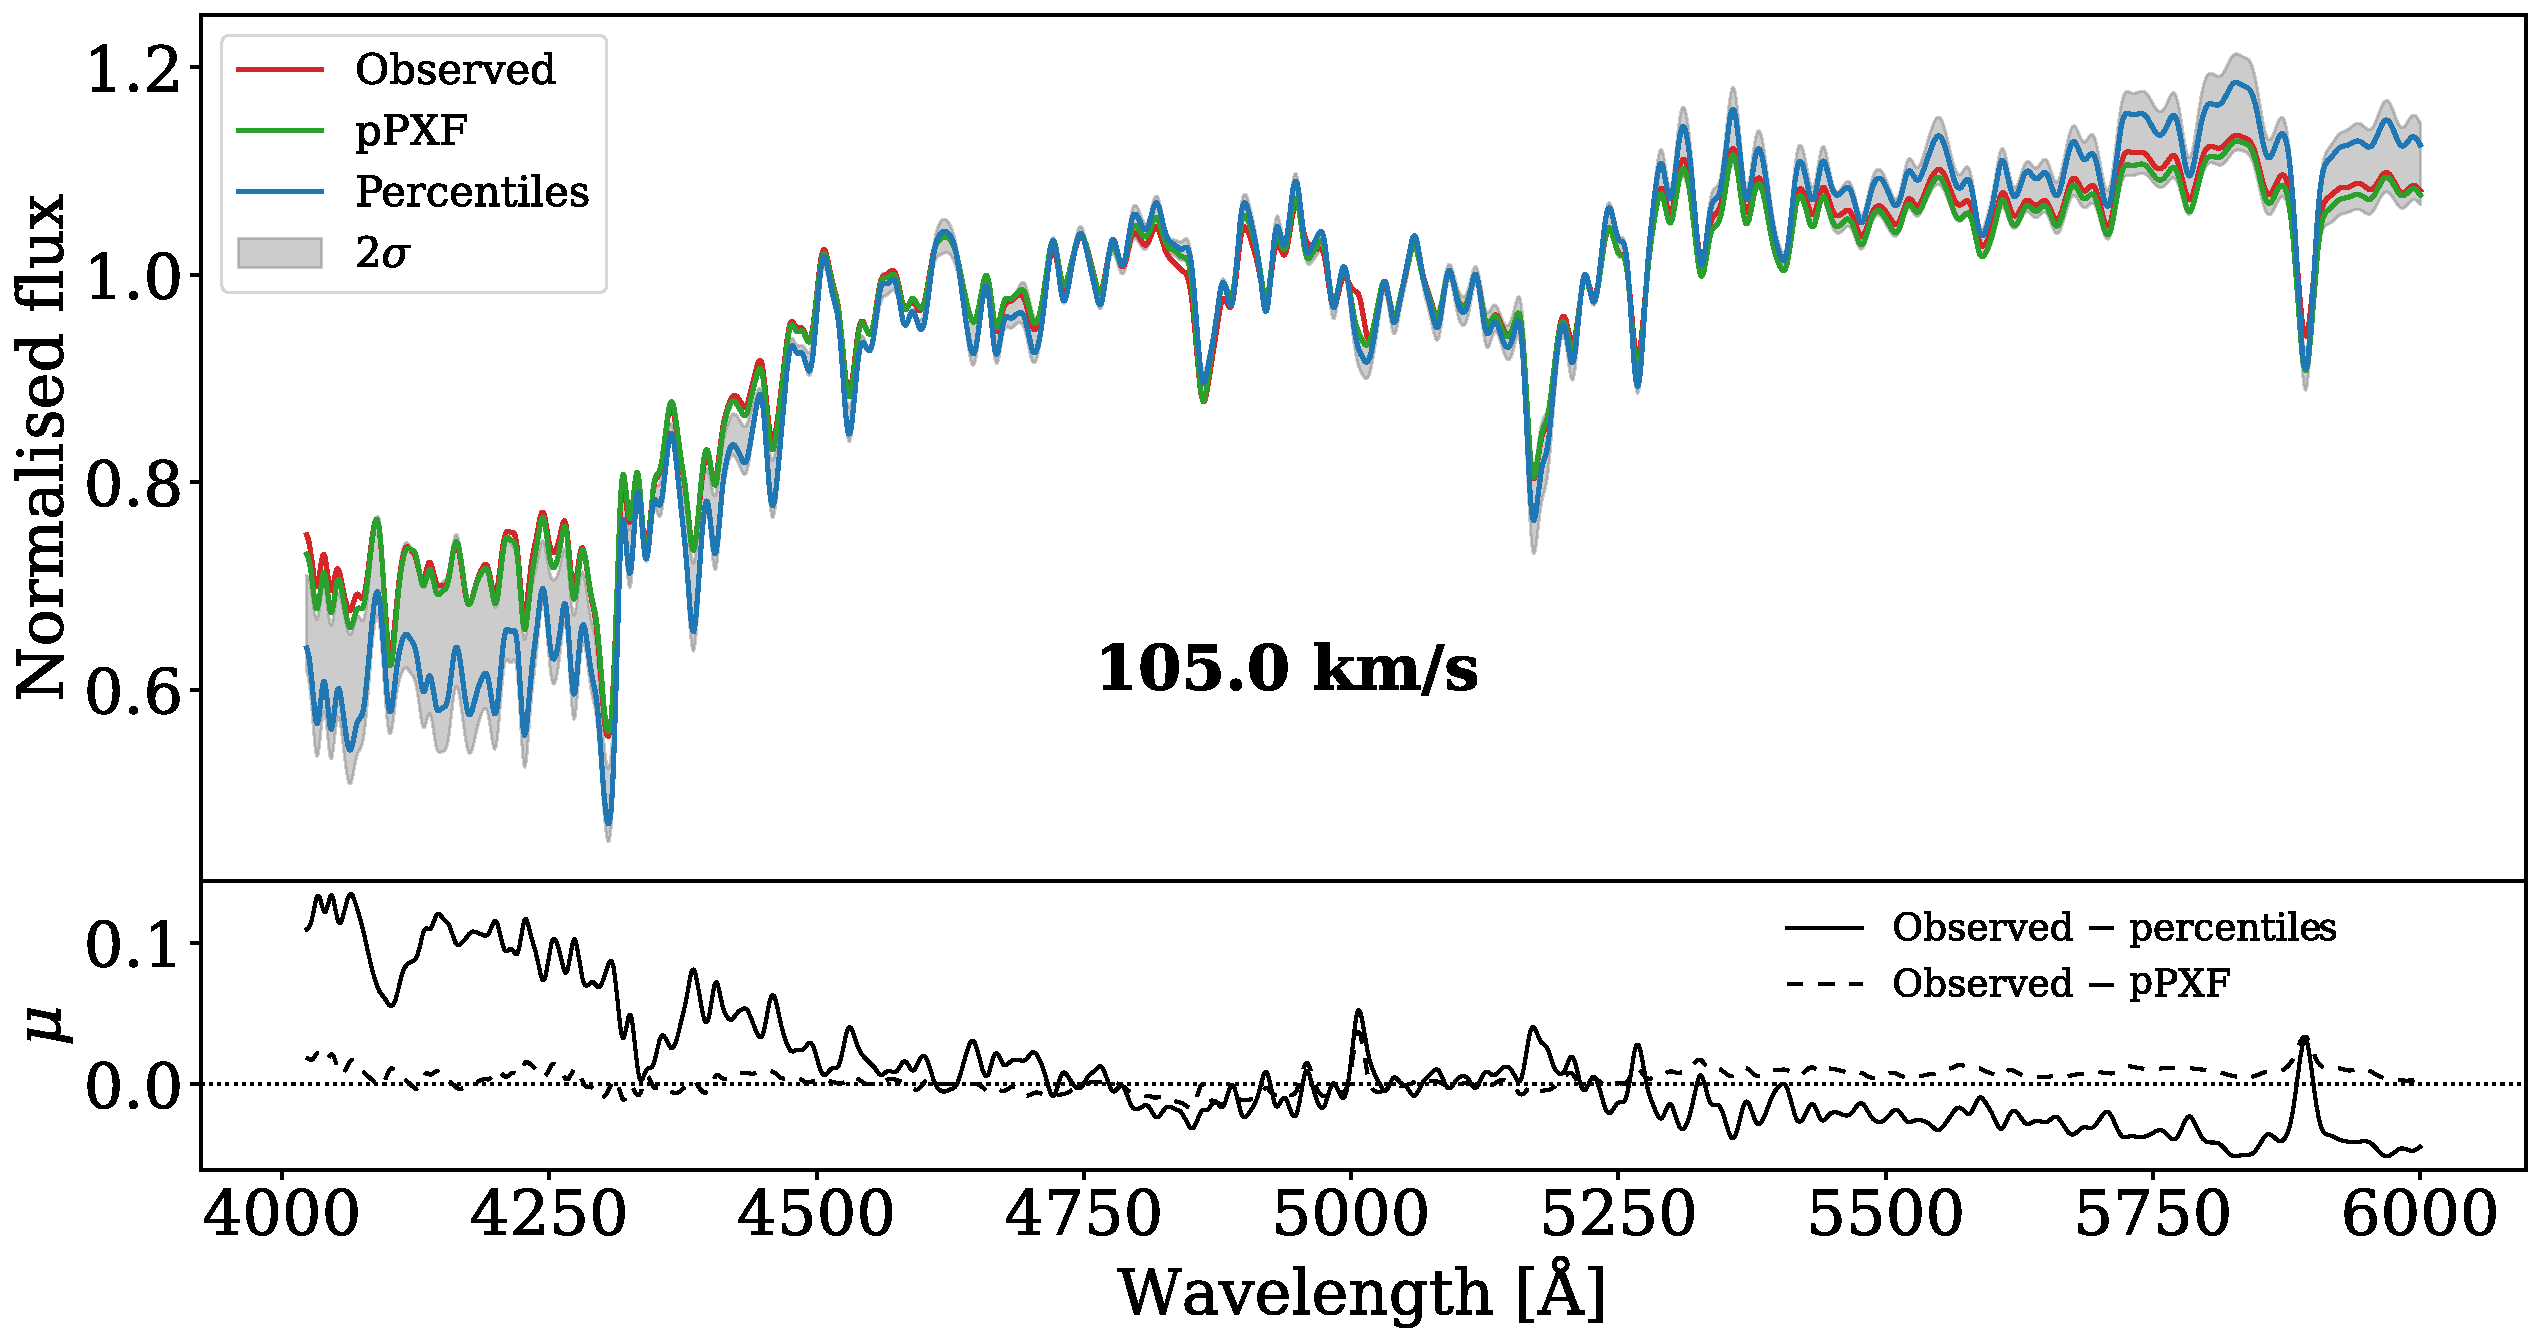
\includegraphics[width=0.5\textwidth]{images/obs/spectra_105.0_2.pdf}
    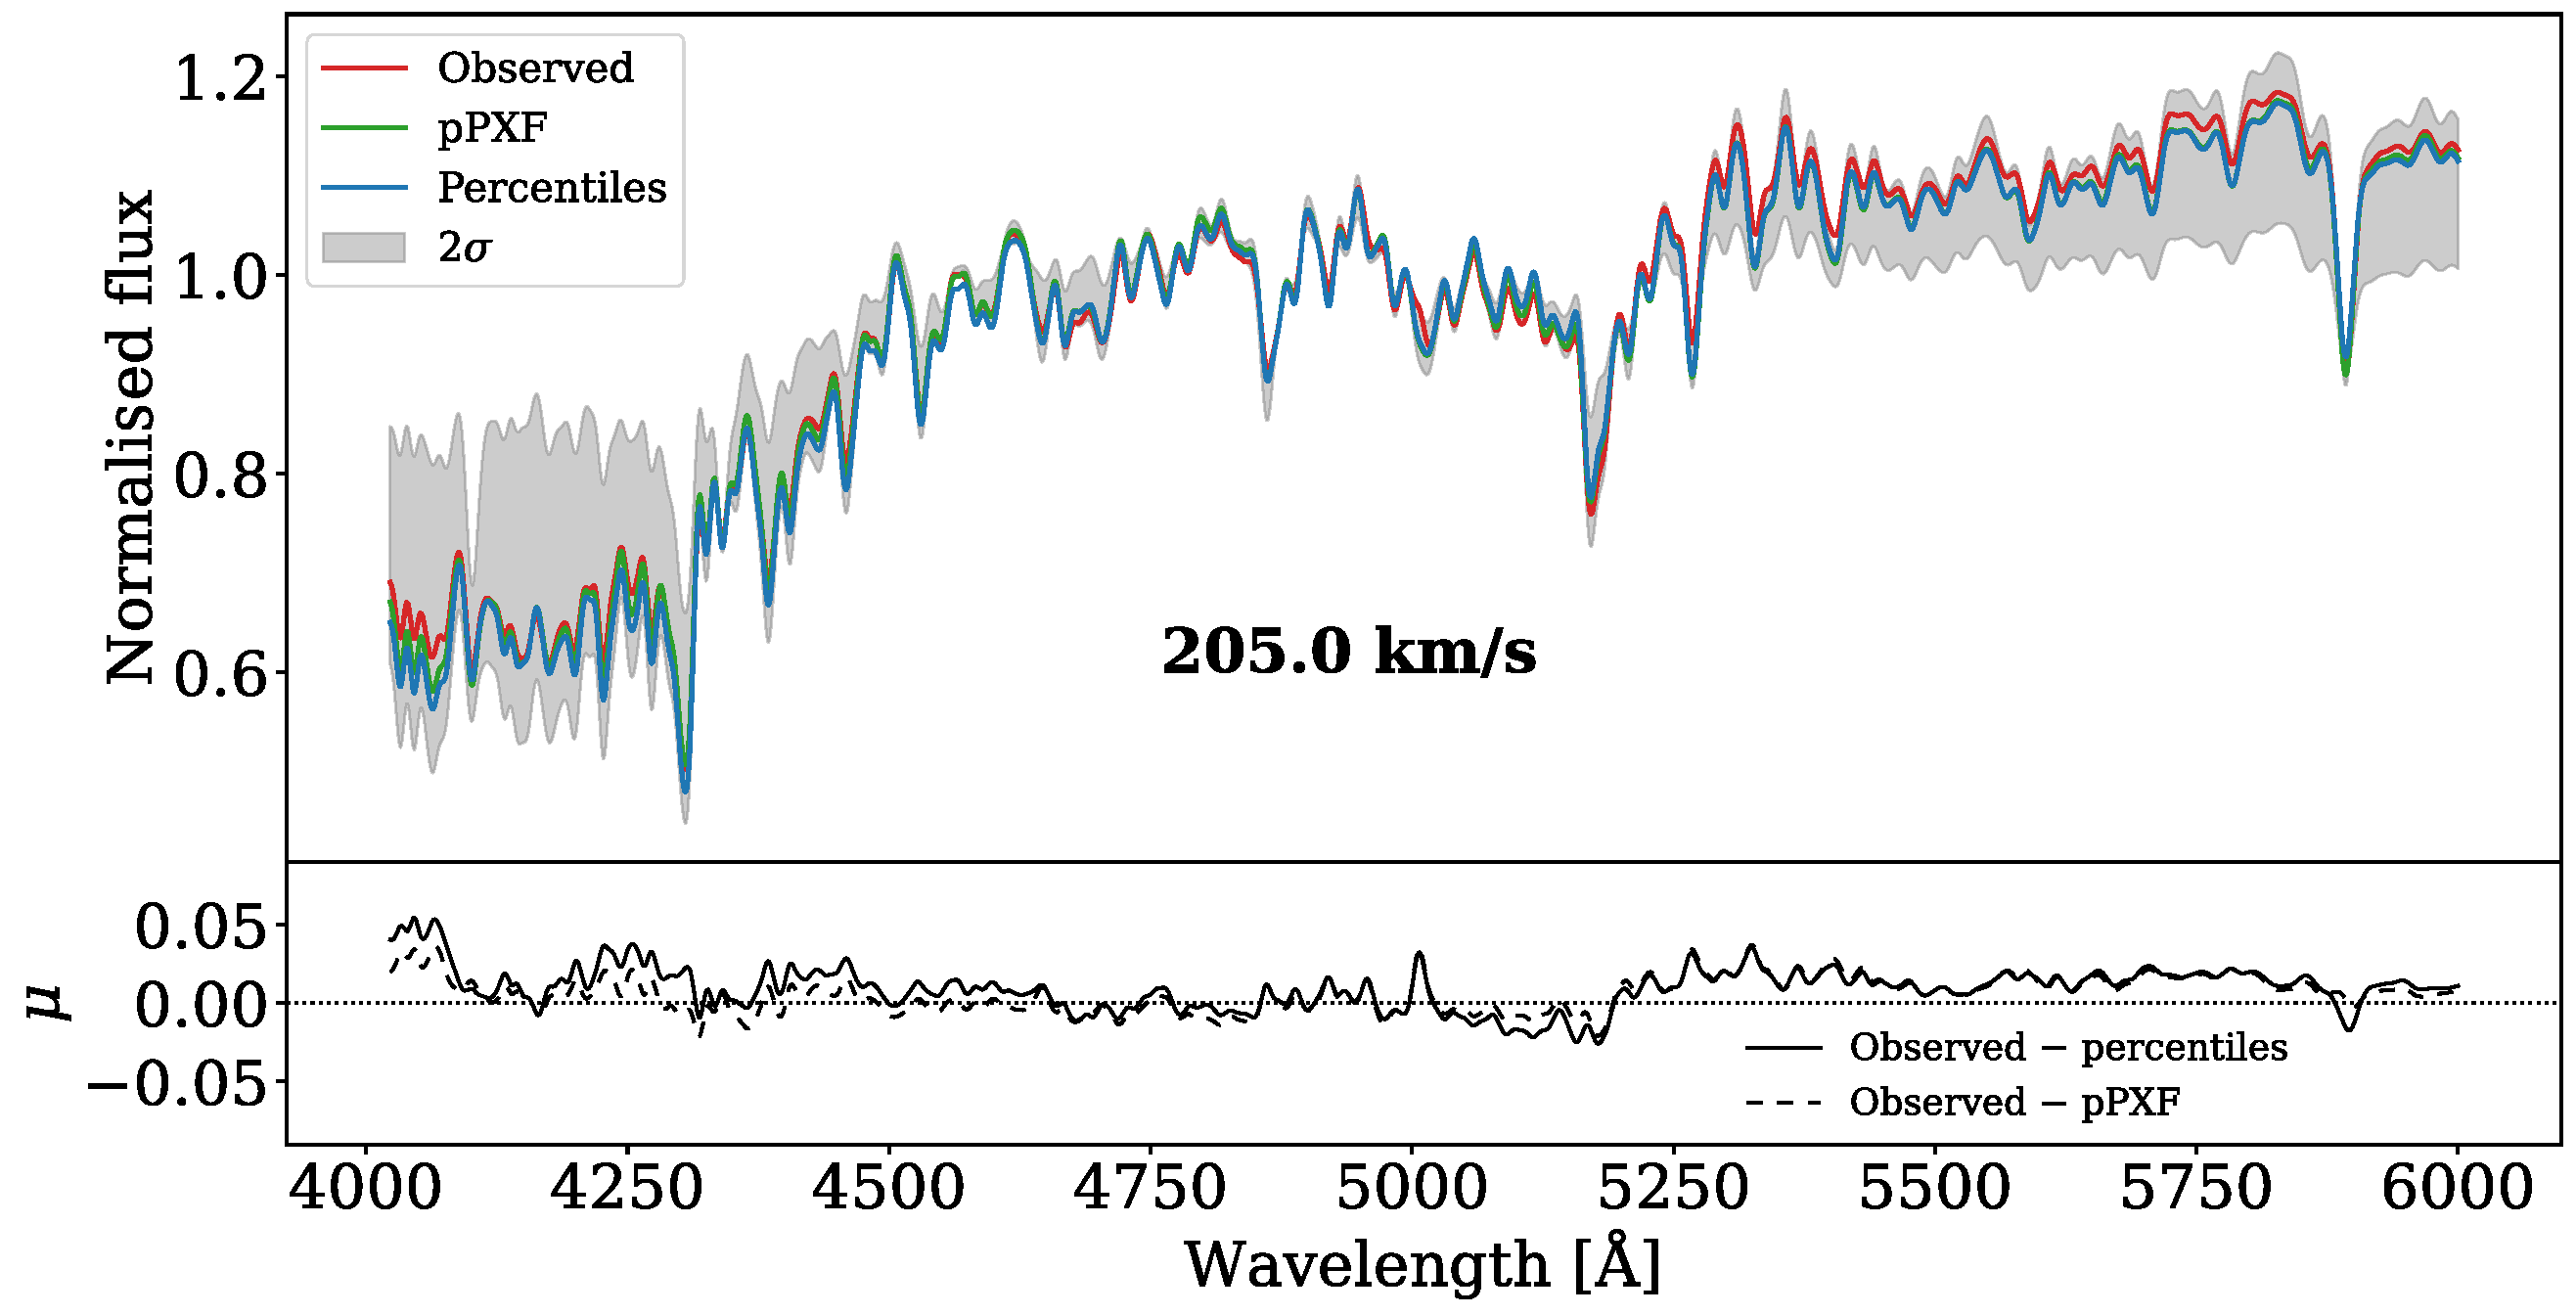
\includegraphics[width=0.5\textwidth]{images/obs/spectra_205.0_2.pdf}
    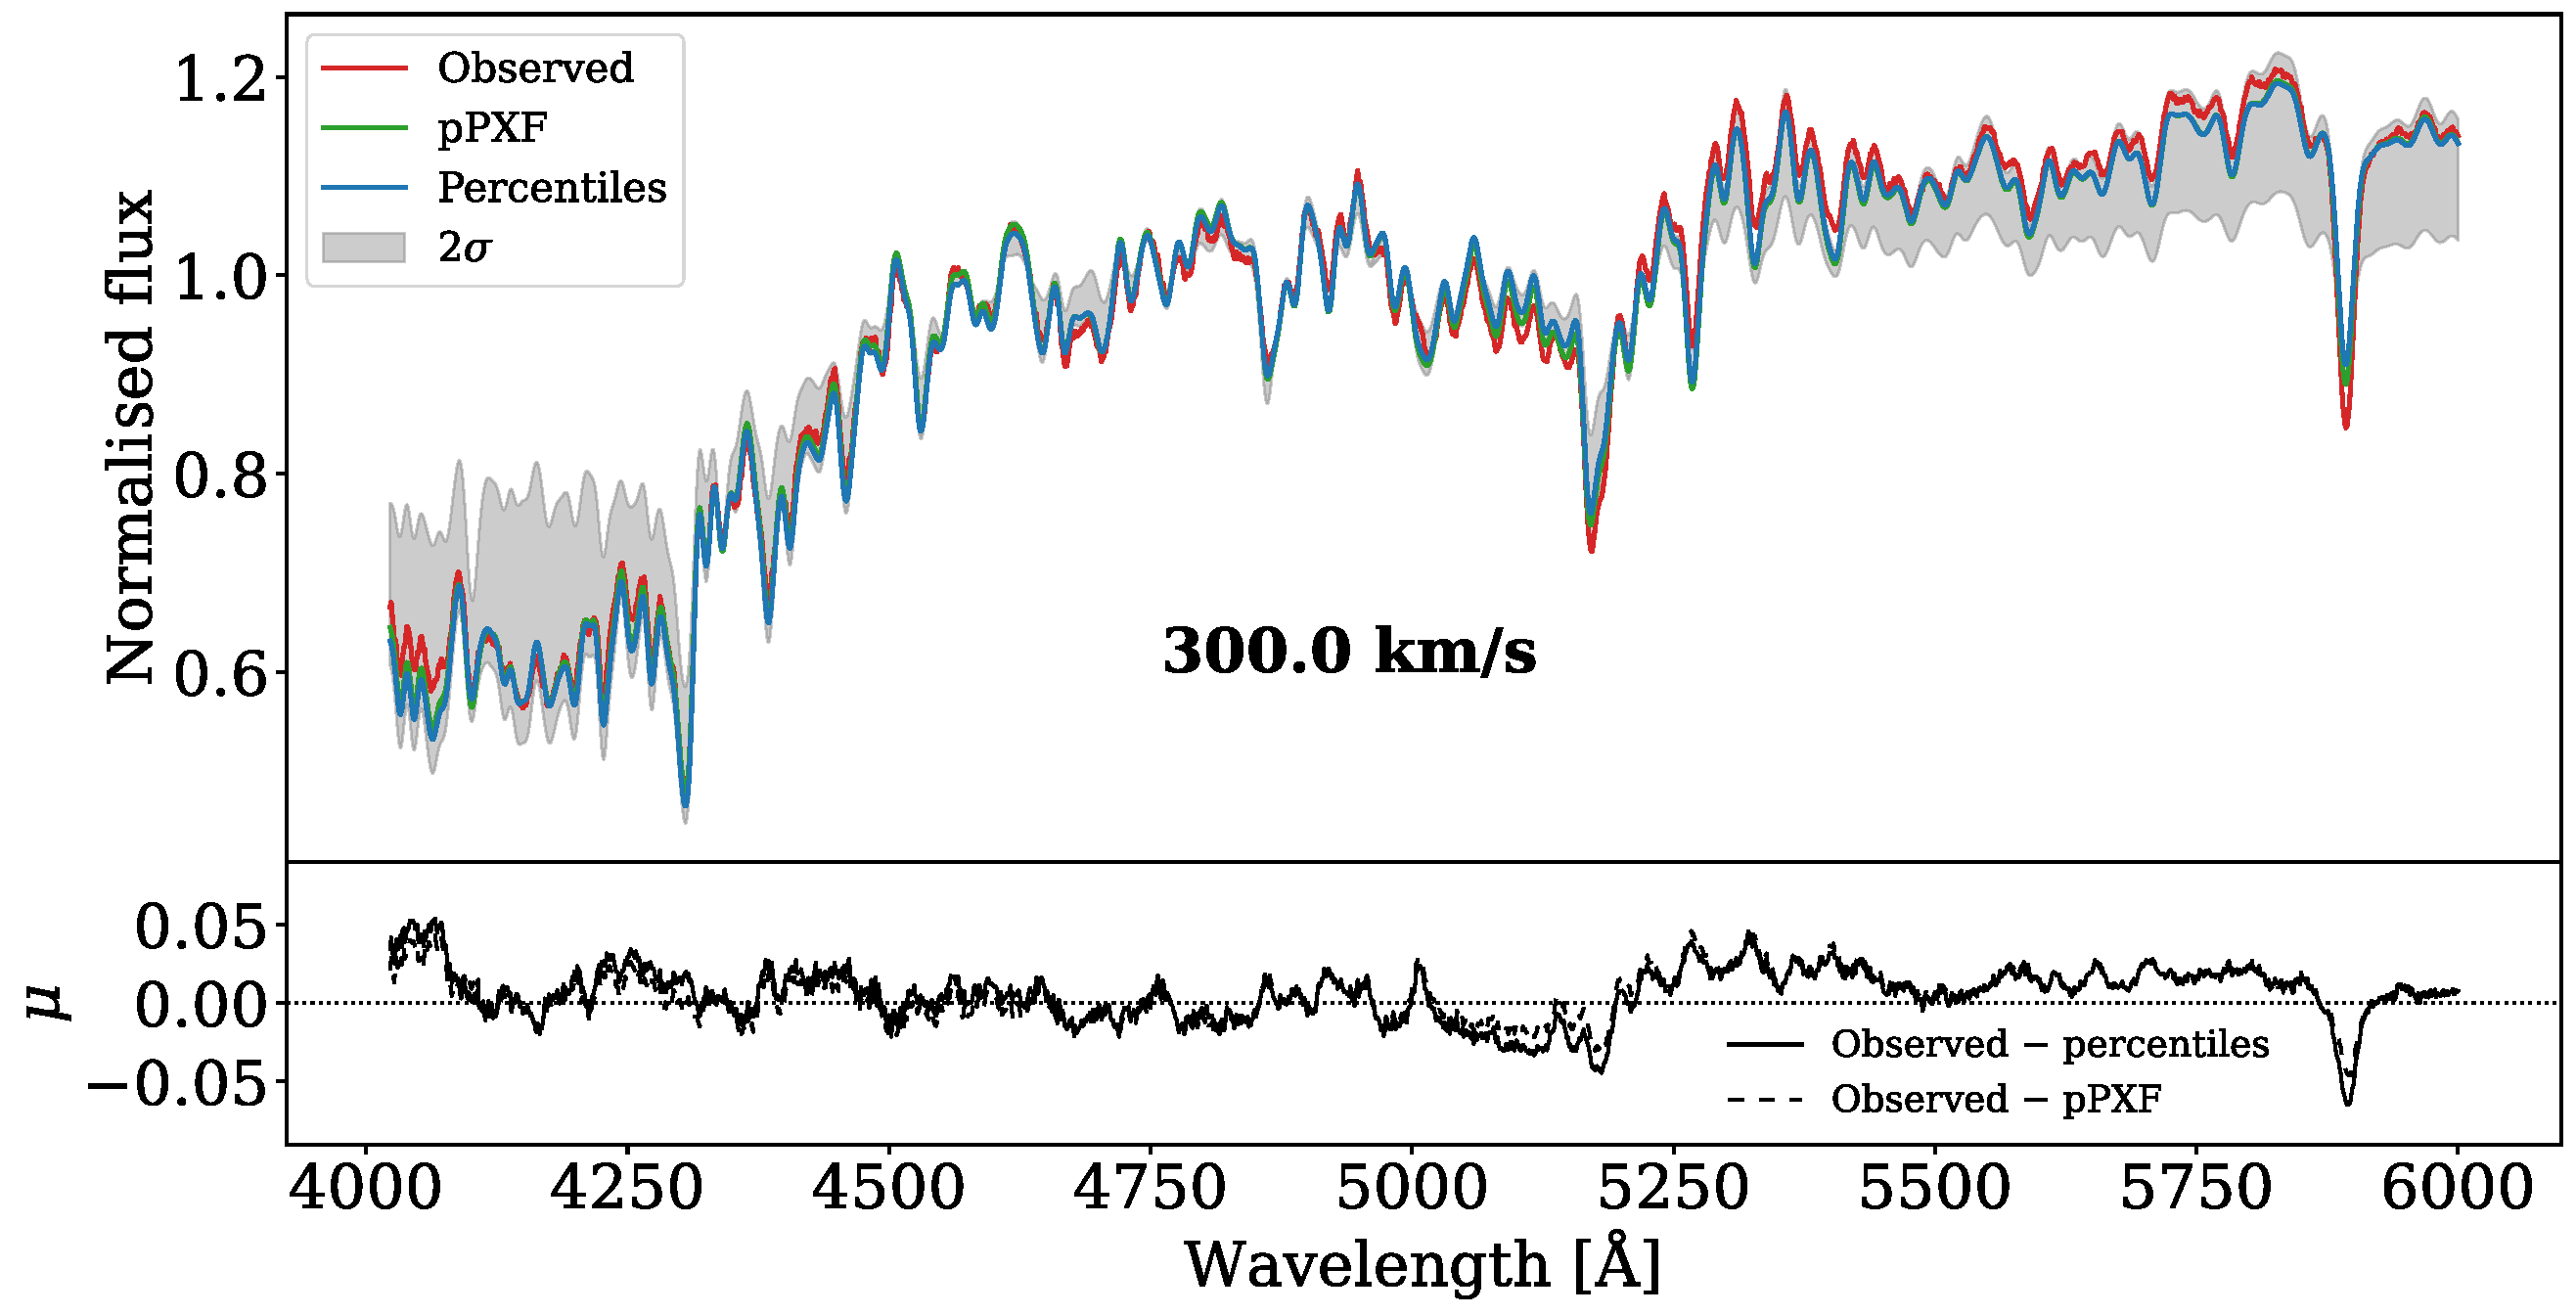
\includegraphics[width=0.5\textwidth]{images/obs/spectra_300.0_2.pdf}
    
    
    \caption{Reconstructions of the observed spectra for the stacks with velocity dispersion $105$, $205$ and $300$ km/s. In red we show the observed spectra, normalised by the median, in the wavelength range $[4023, 6000] \; \AA$. In blue, we show the spectra obtained as a linear combination of MILES SSP spectra according to our model, using the median values of the posteriors predicted. We repeat the procedure for the median $\pm2\sigma$ to get the grey-shadowed stripe, that shows how the uncertainties in the quantities measured are manifested in the spectra. In green, we plot the spectra obtained with the weights given by pPXF. In the lower panels, we include the residuals between the observed spectra and those reconstructed from the percentiles and metallicity predicted by our model (solid black line), and between the observed spectra and the one recovered by pPXF (dashed black line). The dotted line indicates the zero level. The typical value of the residuals of our method $(1.7\%)$ is very similar to the average value obtained with pPXF $(1.5\%)$, although in the first case the inference is performed in the latent space, without directly trying to reproduce the observed spectra.}
    \label{spectra_obs}
\end{figure}





